\chapter{Experimentação e resultados}
\label{cap:experiments}

\section{Ambiente de simulação}

Uma simulação da rede nacional de pesquisa, a rede Ipê \citep{ipe2015network} 
foi criada em laboratório.
Um comutador (\emph{switch}) OpenFlow e quatro servidores foram utilizados 
para executar a simulação no laboratório WiNet \citep{winet22015lab}
no departamento de Ciência da Computação (DCC) da Universidade Federal 
de Minas Gerais (UFMG).

\subsection{A rede Ipê}
Operada pela Rede Nacioanal de Pesquisa (RNP), a rede Ipê é uma infraestrutura
de rede Internet dedicada à comunidade de pesquisa brasileira.
Inaugurada em 2005, foi a primeira rede óptica nacional acadêmica a entrar em
operação na América Latina.

A rede IPÊ implementa 27 Pontos de Presença (\emph{POPs}), um para cada unidade
da federação.
Em cada unidade existem diversos clientes que, para se comunicar com outras 
máquinas em outros Pontos de Presença, transmitem seus pacotes através do 
POP ao qual atuam como clientes.
Essas ramificações constituem mais de 800 instituições de ensino, saúde e 
pesquisa em todo o país, beneficiando mais de 3,5 milhões de usuários
\citep{ipe2015network}.

Através da rede RedCLARA \citep{redclara2015network}, a rede Ipê se conecta 
à 2,5 Gb/s com, atualmente, 15 países da América Latina e à 5 Gb/s com a rede
europeia Géant \citep{geant2015network}. 
Além disso, por meio de quatro conexões de
10 Gb/s, duas pelo Oceano Atlântico e duas pelo Oceano Pacífico, 
operadas em parceria com a ANSP, totalizando 40 Gb/s, a rede Ipê se conecta 
às redes acadêmicas norte-americanas, em especial, a  Internet2 
\citep{internet22015network}, a outras redes acadêmicas internacionais e à 
internet comercial mundial.

Os Pontos de presença estão interconectados conforme mostrado na figura 
\ref{fig:ipe-network-2015}.

\begin{figure}[!ht]
    \centering
    \label{fig:ipe-network-2015}
    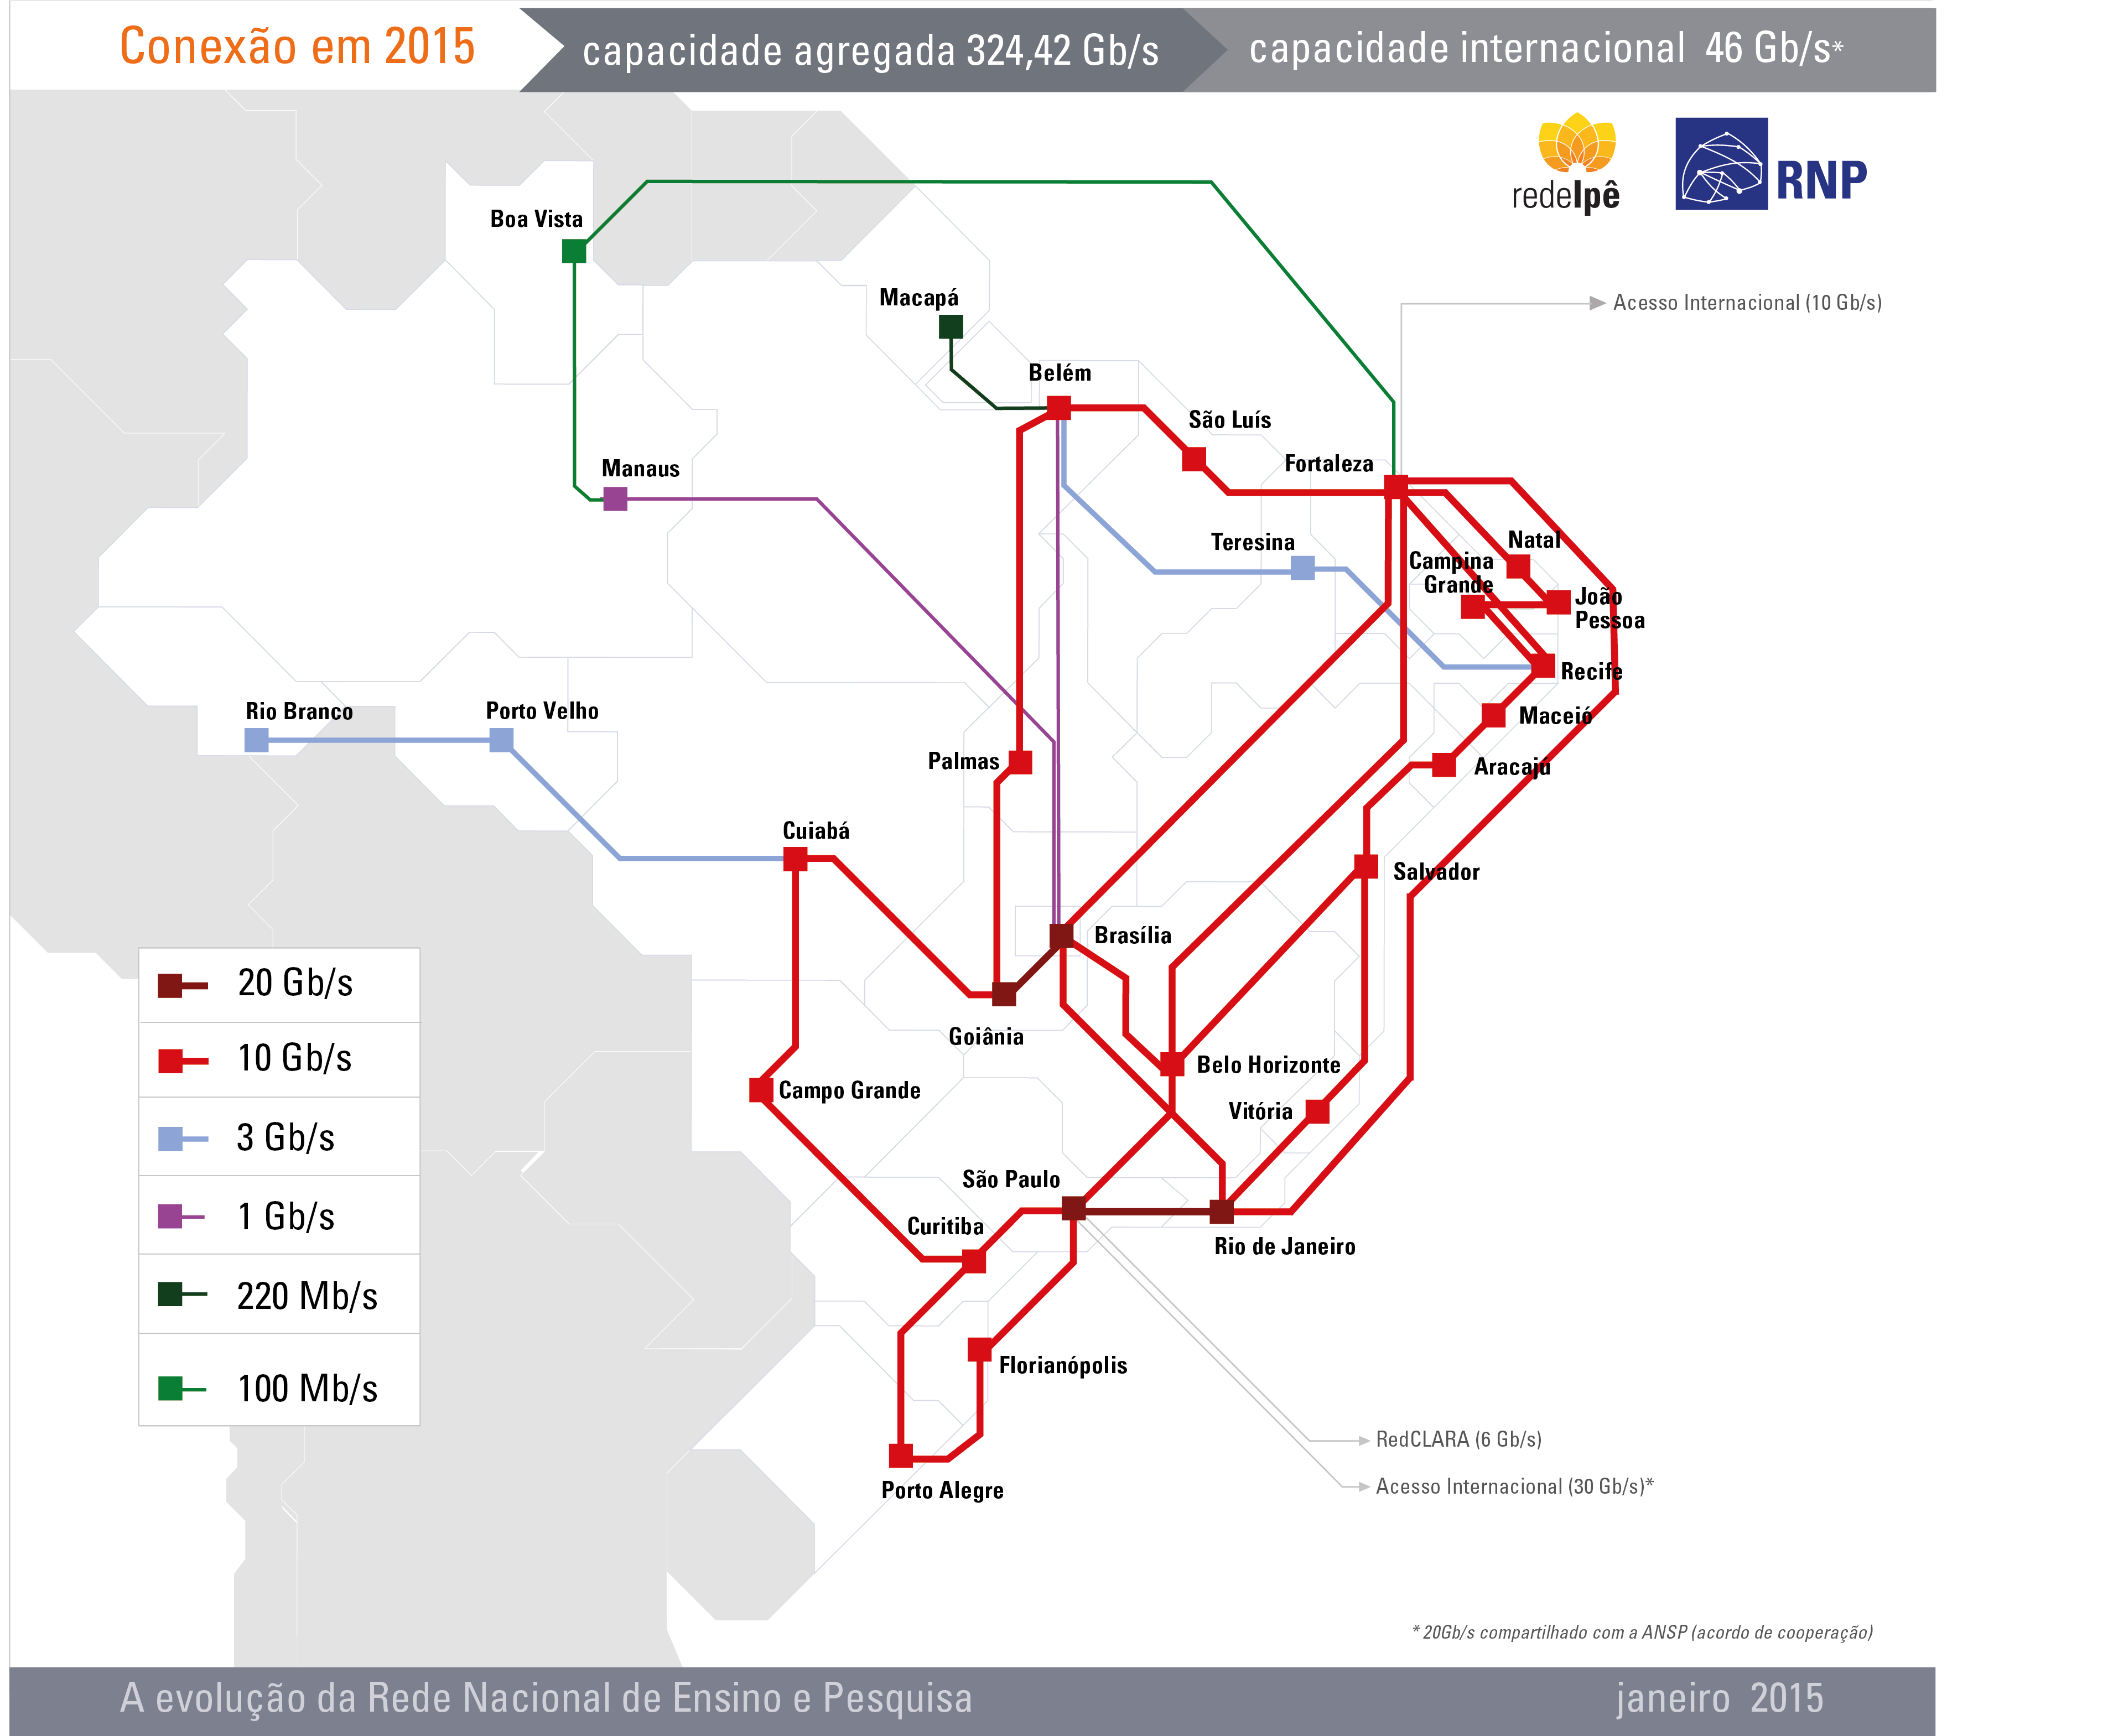
\includegraphics[width=\textwidth]{img/ipe-network-2015}
    \caption{Rede Nacional de Pesquisa IPÊ \protect\footnotemark}
    \vspace*{3in}
\end{figure}

\footnotetext{Imagem retirada de 
\url{http://www.rnp.br/servicos/conectividade/rede-ipe}}

\subsection{Arquitetura da simulação}

A ambiente de simulação é composto por um comutador HP com OpenFlow habilitado.
Quatro servidores são responsáveis por gerenciar máquinas virtuais que 
representam as unidades federativas e suas instituições clientes.

Conforme pode ser visto na figura \ref{fig:physical-vs-virtual-network}, a
rede física do esperimento é separada da rede virtual.
O quinto computador é o controlador da rede. 
Para o experimento, existem duas redes. 
Uma rede de administração, com acesso aos servidores e a uma instância do 
controlador, na porta 6633.
A segunda rede é a rede virtual à qual todos os POPs simulados estão 
conectados. 
Para implementar essas duas redes, cada servidor e o controlador possuem duas
interfaces de rede que isolam seus funcionamentos.
Assim, a rede física/administrativa e a rede virtual/Ipê estão separadas
em nosso experimento.


\begin{figure}[!h]
    \centering
    \label{fig:physical-vs-virtual-network}
    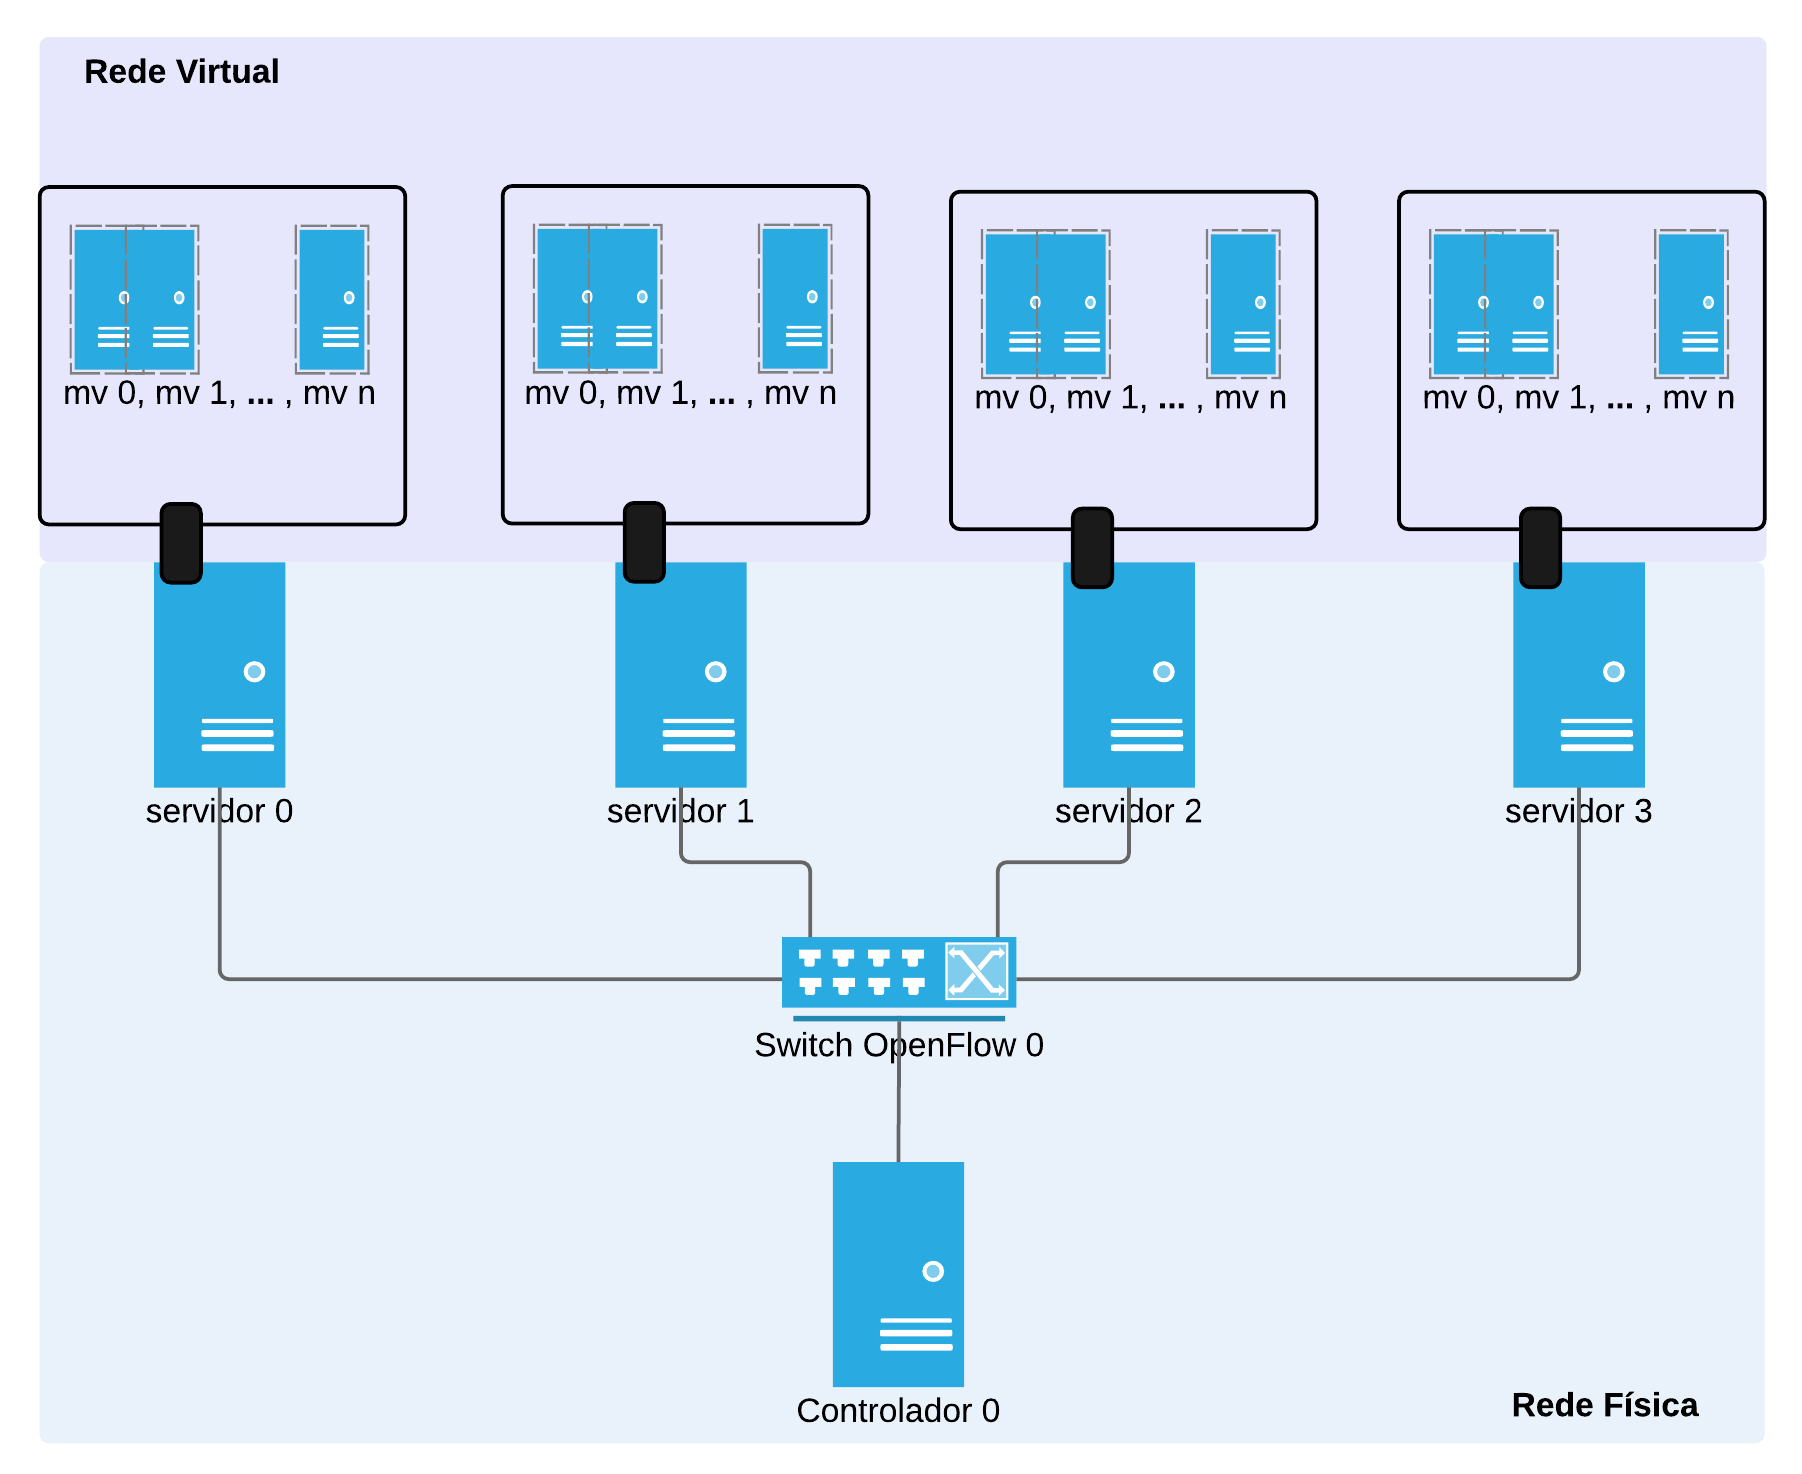
\includegraphics[width=\textwidth]{img/physical-vs-virtual-network-pt}
    \caption{Arquitetura do ambiente de simulação}
\end{figure}

Para o ambiente virtualizado, o controlador está associado a porta 6653.
Cada POP é um comutador (\emph{switch}) OpenFlow simulado via OpenVSwitch
\citep{openvswitch2015switch}.
As instituições clientes de cada POP são simuladas através do \emph{Mininet} 
\citep{lantz2010network}.
O número de instituições clientes foi coletado do sítio de cada Ponto de 
Presença.

Cada máquina virtual representa um POP.
Cada POP possui uma subrede à qual uma instância do \emph{Mininet} simula 
seus clientes. 
Essa subrede está conectada através de um \emph{switch} virtual 
\emph{OpenVSwitch} que é controlado pelo controlador da rede virtualizada.
Assim, para cada POP, temos as decisões e atualizações da tabela de fluxos
feita pelo controlador.
Toda comunicação de saída das subredes utilizando \emph{mininet} passam pelo 
\emph{OpenVSwitch} que funciona em modo \emph{bridge} (ponte) com a interface
de rede virtual conforme pode ser visto na figura
\ref{fig:mininet-vm-architecture}.


\begin{figure}[h!]
    \centering
    \label{fig:mininet-vm-architecture}
    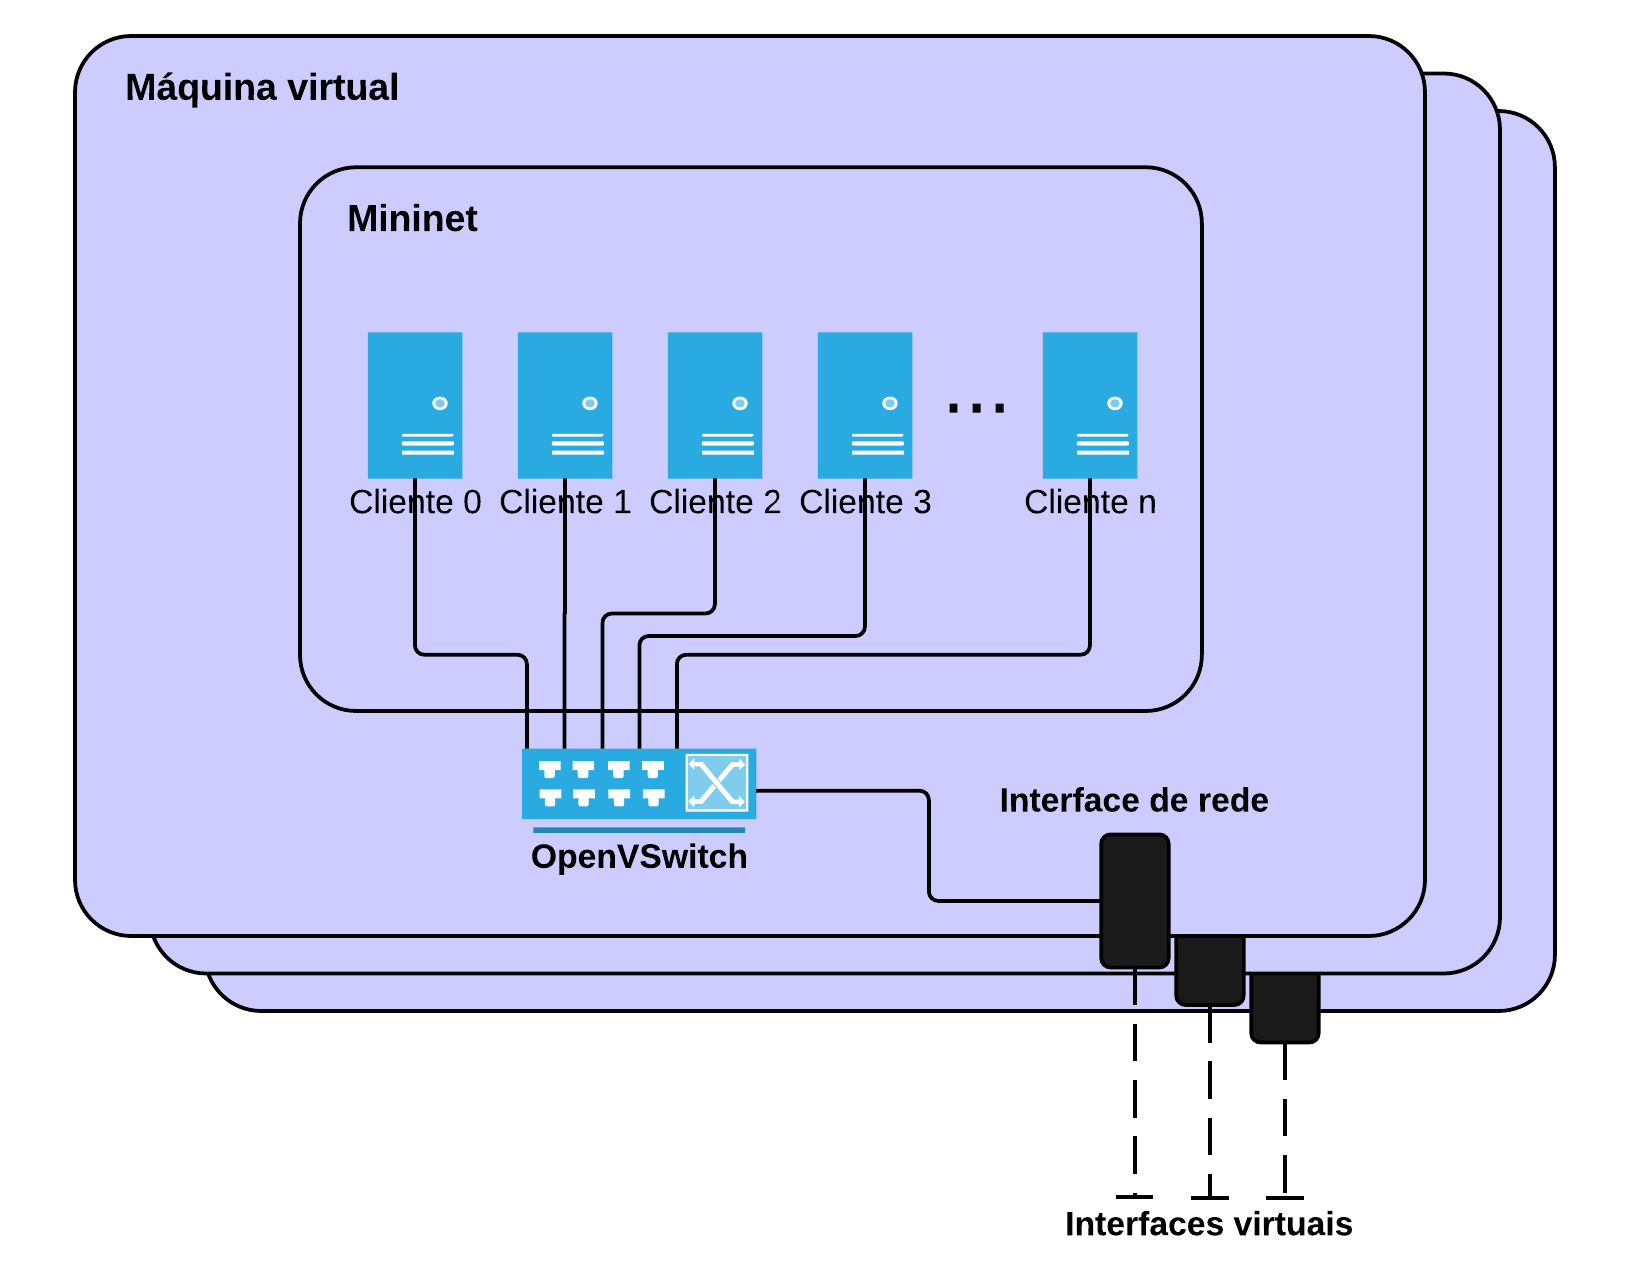
\includegraphics{img/mininet-vm-architecture}
    \caption{Arquitetura de cada máquina virtual}
\end{figure}


A tabela \ref{tbl:testbed-ipe-net} apresenta as subredes de cada unidade
federativa (POP), qual servidor físico gerencia a máquina virtual referente
ao POP e o número de clientes a ele associado.

\begin{table}[h]
    \label{tbl:testbed-ipe-net}
    \centering
    \resizebox*{!}{\dimexpr\textheight- 25px}{
    \resizebox{\linewidth}{!}{
    \begin{tabular}{llllll}
        \rowcolor[HTML]{000000} 
        \multicolumn{6}{c}{\cellcolor[HTML]{000000}{\color[HTML]{C0C0C0} 
            \textbf{Associação de Servidores à simulação da rede IPÊ}}} \\
        \rowcolor[HTML]{000000} 
        {\color[HTML]{9B9B9B} \textbf{UF}} & {\color[HTML]{9B9B9B} 
            \textbf{N clientes}} & {\color[HTML]{9B9B9B} 
            \textbf{Sub-rede local}} & {\color[HTML]{9B9B9B} 
            \textbf{Servidor}} & {\color[HTML]{9B9B9B} \textbf{IP local}} & 
            {\color[HTML]{9B9B9B} \textbf{IP Gateway}} \\
        AC &  10 &  10.10.1.0 &   Shiva  &  10.10.42.51 & \\ 
        AL  & 13 &  10.10.2.0  &  Shiva  &  10.10.42.52 & \\ 
        AM  & 20 &  10.10.3.0 &   Shiva  &  10.10.42.53 & \\
        AP  & 7  &  10.10.4.0 &   Shiva  &  10.10.42.54 & 10.10.42.50 \\
        BA  & 25 &  10.10.5.0 &   Shiva  &  10.10.42.55 & \\
        CE  & 50  & 10.10.6.0  &  Shiva  &  10.10.42.56 & \\
        DF  & 16 &  10.10.7.0  &  Shiva  &  10.10.42.57 & \\ \hline
        ES  & 26  & 10.10.8.0  &  Eden  &   10.10.42.101 & \\
        GO  & 26  & 10.10.9.0  &  Eden  &   10.10.42.102  & \\  
        MA  & 7  &  10.10.10.0 &  Eden  &   10.10.42.103  & \\  
        MG  & 32  & 10.10.11.0  & Eden  &   10.10.42.104  & 10.10.42.100 \\  
        MS  & 10  & 10.10.12.0  & Eden  &   10.10.42.105  & \\  
        MT  & 8   & 10.10.13.0  & Eden  &   10.10.42.106  & \\  
        PA  & 13  & 10.10.14.0  & Eden  &   10.10.42.107  & \\ \hline
        PB  & 14  & 10.10.15.0  & Diablos & 10.10.42.151  & \\
        PE  & 41  & 10.10.16.0  & Diablos & 10.10.42.152  & \\  
        PI &  25 &  10.10.17.0 &  Diablos & 10.10.42.153  & \\  
        PR &  71 &  10.10.18.0 &  Diablos & 10.10.42.154  & 10.10.42.150 \\
        RJ &  27 &  10.10.19.0 &  Diablos & 10.10.42.155  & \\  
        RN &  11 &  10.10.20.0 &  Diablos & 10.10.42.156  & \\  
        RO &  10 &  10.10.21.0 &  Diablos & 10.10.42.157  & \\ \hline
        RR  & 7  &  10.10.22.0 &  Leviathan &   10.10.42.201 & \\
        RS &  10 &  10.10.23.0 &  Leviathan &   10.10.42.202  & \\  
        SC &  47 &  10.10.24.0 &  Leviathan &   10.10.42.203 & 10.10.42.200 \\   
        SE &  13 &  10.10.25.0 &  Leviathan &   10.10.42.204 & \\   
        SP &  25 &  10.10.26.0 &  Leviathan &   10.10.42.205  & \\  
        TO &  11 &  10.10.27.0 &  Leviathan &   10.10.42.206 & \\   
    \end{tabular}
    }}
\end{table}



\section{Detecção de entidades}

Ao ser carregado, o módulo \emph{graph} inicia o grafo da rede vazio.
Os \emph{switches} são os primeiros a serem identificados. 
Como o controlador está ligado diretamente a eles pela interface
\emph{OpenFlow}, um evento de \emph{ConnectionUp} é disparado 
pelo núcleo do controlador.
Esse evento dispara o evento \emph{SwitchJoin} através do módulo 
\emph{topology} que faz com que o grafo adicione vértices.

\begin{figure}[h!]
    \centering
    \begin{lstlisting}[ tabsize=4,  
                        language=bash,
                        basicstyle=\ttfamily\footnotesize,
                        aboveskip={1.5\baselineskip},
                        columns=fixed,
                        showstringspaces=false,
                        extendedchars=true,
                        breaklines=true,
                        frame=single,
                        numbers=left,
                        showtabs=false,
                        showspaces=false,
                        showstringspaces=false,
                        identifierstyle=\ttfamily,
                        ]
INFO:topology.graph:SwitchJoin id: 2
INFO:topology.graph:SwitchJoin id: 1
INFO:topology.graph:1, 2
DEBUG:openflow.discovery:Dropping LLDP packet 275
INFO:topology.graph:LinkEvent fired
INFO:host_tracker:Learned 1 1 7e:e6:9b:89:39:2e got IP 10.0.0.1
INFO:topology.graph:HostJoin id: 7e:e6:9b:89:39:2e
INFO:host_tracker:Learned 2 1 62:77:44:24:13:49 got IP 10.0.0.2
INFO:topology.graph:HostJoin id: 62:77:44:24:13:49
        \end{lstlisting}
    \caption{Detecção de entidades}
    \label{fig:detection}
\end{figure}

Nas duas primeiras linhas do \emph{log} mostrado na figura
\ref{fig:detection}, o módulo \emph{graph} foi notificado
da descoberta de dois \emph{switches} na rede.
Na linha 5, nota-se a descoberta de um enlace (\emph{link}) entre dois
comutadores (\emph{switches}).
O módulo \emph{openflow.discovery}, através do protocolo LLDP identificou 
o link entre \emph{switches}.
O grafo foi notificado e estabeleceu uma aresta entre os 
vértices (\emph{switches}).

As linhas 7 e 9 mostram a descoberta de dois hosts.
Esses hosts foram descobertos pelo módulo \emph{host\_tracker} via 
escuta dos eventos de DHCP.
É importante ressaltar que a descoberta de \emph{hosts} também ocorre 
independente do DHCP.
Um novo pacote que passa por um \emph{switch} e não possui regra
instalada na tabela de fluxos é encaminhado ao controlador que 
dispara um evento de \emph{PacketIn}. 
Para tal, o \emph{host\_tracker} se encarrega de escutar esse evento 
e notificar o grafo através do evento \emph{HostJoin} disparado pelo módulo
\emph{topology} ao criar um novo \emph{Host}.
O grafo, ao ser notificado, cria vértices para esses \emph{hosts} associando 
uma aresta entre eles e o \emph{switch} ao qual eles estão conectados.
Dessa forma as entidades da rede são identificadas e computadas no grafo.


\section{Remoção de entidades}

\subsection{Remoção de computadores}

Diversos computadores foram desligados de maneira aleatória.
O \emph{host\_tracker}, após um tempo fixo (\emph{timerInterval}) 
verifica via ARPPing se os \emph{hosts} conhecidos estão ativos.
Para esse cenário da remoção de um computador (\emph{host}), 
o \emph{host\_tracker} identifica a inatividade do \emph{host} e remove o 
\emph{Host}.
O evento de \emph{HostLeave} é disparado pelo \emph{topology}, 
atualizando assim o grafo.

Nesse cenário de experimento, cinco computadores de cada subrede foi desligado.
Para cada computador foi coletado o tempo em que ele foi desligado.
Quando o controlador, através do \emph{host\_tracker}, identifica a saída 
desse computador o tempo é novamente coletado.
Assim, para cada computador desligado, foi computado o tempo decorrido até 
que o controlador o removesse do grafo da rede.

\begin{figure}[h!]
    \centering
    \label{fig:hosts-leave-time}
    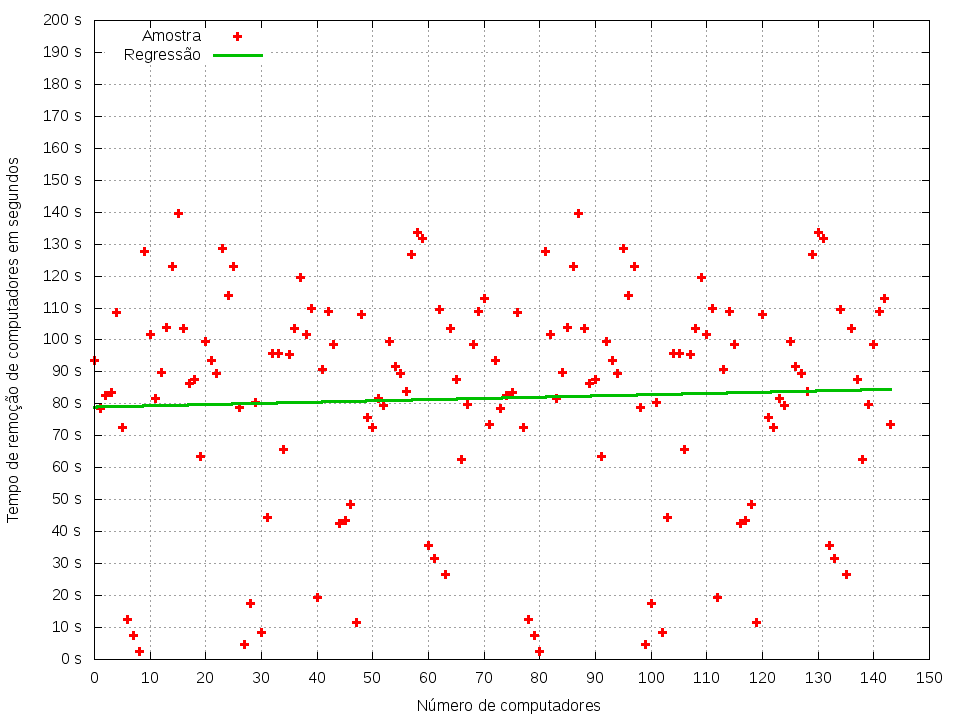
\includegraphics[width=\linewidth]{img/hosts-leave-time}
    \caption{Tempo decorrido entre o desligamento de um computador e a 
    remoção do mesmo no grafo}
\end{figure}

Os resultados da amostra coletada pode ser visto na figura
\ref{fig:hosts-leave-time}.
Em média, o tempo de remoção de um computador do grafo demorou 80 segundos.
A sondagem foi configurada para ser executada com uma periodicidade de 60 
segundos. 
A regressão linear computada mostra que esse valor médio é praticamente 
constante ao longo dos valores amostrados.

Computadores cuja remoção ocorreram em um intervalo de tempo muito reduzido
tiveram seu tempo de sondagem expirado muito próximos ao momento em que 
o \emph{host\_tracker} executava sua sondagem. 

\subsection{Remoção de comutadores}

Para o caso de comutadores (\emph{switch}), foram desligados os 
\emph{switches} e medido o tempo de atualização do grafo.
O controlador está ligado diretamente aos \emph{switch}. 
Em função disso os comutadores são removidos mais rapidamente do grafo.
A figura \ref{fig:switch-leave-time} apresenta os resultados da 
computação da amostra de \emph{switches} removidos.
Assim, ao ser desligado, o \emph{core} do POX dispara um evento 
de \emph{SwitchLeave} ao qual o módulo \emph{graph} está inscrito. 
Logo, o grafo é atualizado removendo o vértice do \emph{switch}.

\begin{figure}[h!]
    \centering
    \label{fig:switch-leave-time}
    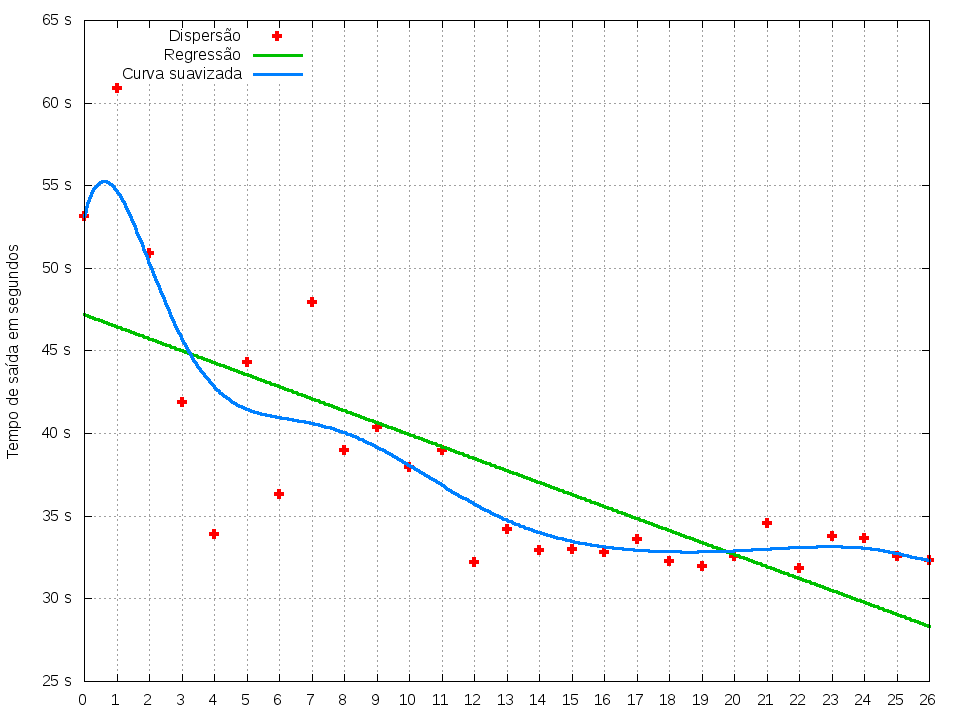
\includegraphics[width=\linewidth]{img/switch-leave-time}
    \caption{Tempo decorrido entre o desligamento de um comutador 
    (\emph{switch}) e a remoção do mesmo no grafo}
\end{figure}

Uma curva suavizada da interpolação dos pontos mostra que apesar dos valores
de tempo mais elevados nos primeiros valores da amostra, ao final esses valores
são praticamente constantes, em um valor de 30 a 35 segundos para cada 
remoção.

Após algum tempo o \emph{host\_tracker} identifica se os computadores 
associados ao \emph{switch} removido estão ativos por outra rota. 
Caso negativo, os computadores são removidos do grafo.
Considerando o experimento da remoção dos comutadores (\emph{switches}),
foi computado o tempo decorrido entre a remoção do \emph{switch} e a 
remoção dos computadores na rede interna ao \emph{switch}. 

\begin{figure}[h!]
    \centering
    \label{fig:hosts-behind-switch-time}
    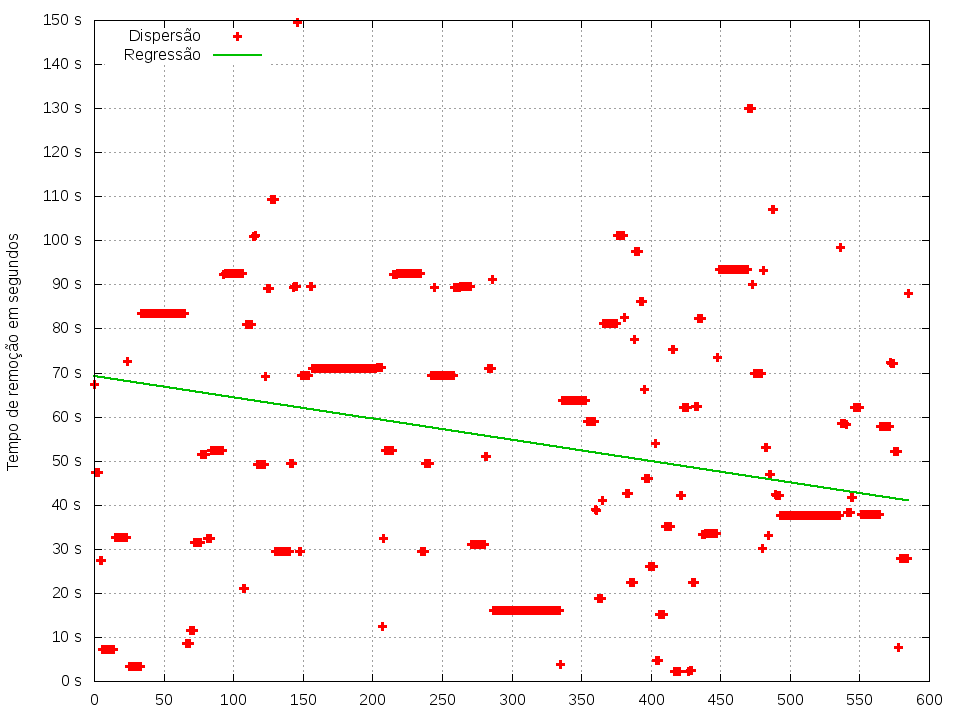
\includegraphics[width=\linewidth]{img/hosts-behind-switch-time}
    \caption{Tempo decorrido entre a remoção dos comutadores 
    (\emph{switches}) e a remoção dos computadores na rede interna ao 
    \emph(switch)}
\end{figure}

A figura \ref{fig:hosts-behind-switch-time} mostra o resultado do experimento
para o tempo de remoção de computadores em função da remoção do 
\emph{switch}.
Os resultados mostram uma média que varia entre 40 e 70 segundos para a 
remoção dos computadores.
No geral nota-se que computadores de uma mesma subrede foram removidos em 
instantes próximos.
Isso pode ser notado pelos pequenos grupos de pontos muito próximos na 
figura.

\section{Visualização em tempo real}

Uma imagem representando o grafo da rede é gerada pelo módulo \emph{graph}.
Essa imagem consiste na representação da topologia da rede no instante 
em que foi gerada. 
Periodicamente uma nova imagem é criada.
Um exemplo de grafo é apresentado na figura \ref{fig:full-graph}.
Essa figura representa uma rede simulada, dentro do ambiente do 
\emph{Mininet}, com 8 comutadores (\emph{switches}), cada um com 30 
computadores (\emph{hosts}) conectados.

Essa topologia totaliza 248 entidades na rede.
Na figura, os vértices vermelhos representam os comutadores.
Os vértices azuis, os computadores.
Cada aresta é um enlace entre dois vértices.

Atualizações na topologia como, remover e adicionar entidades na rede, foram
executados.
A visualização da rede atualiza junto com as alterações no grafo.

\begin{figure}[h!]
    \centering
    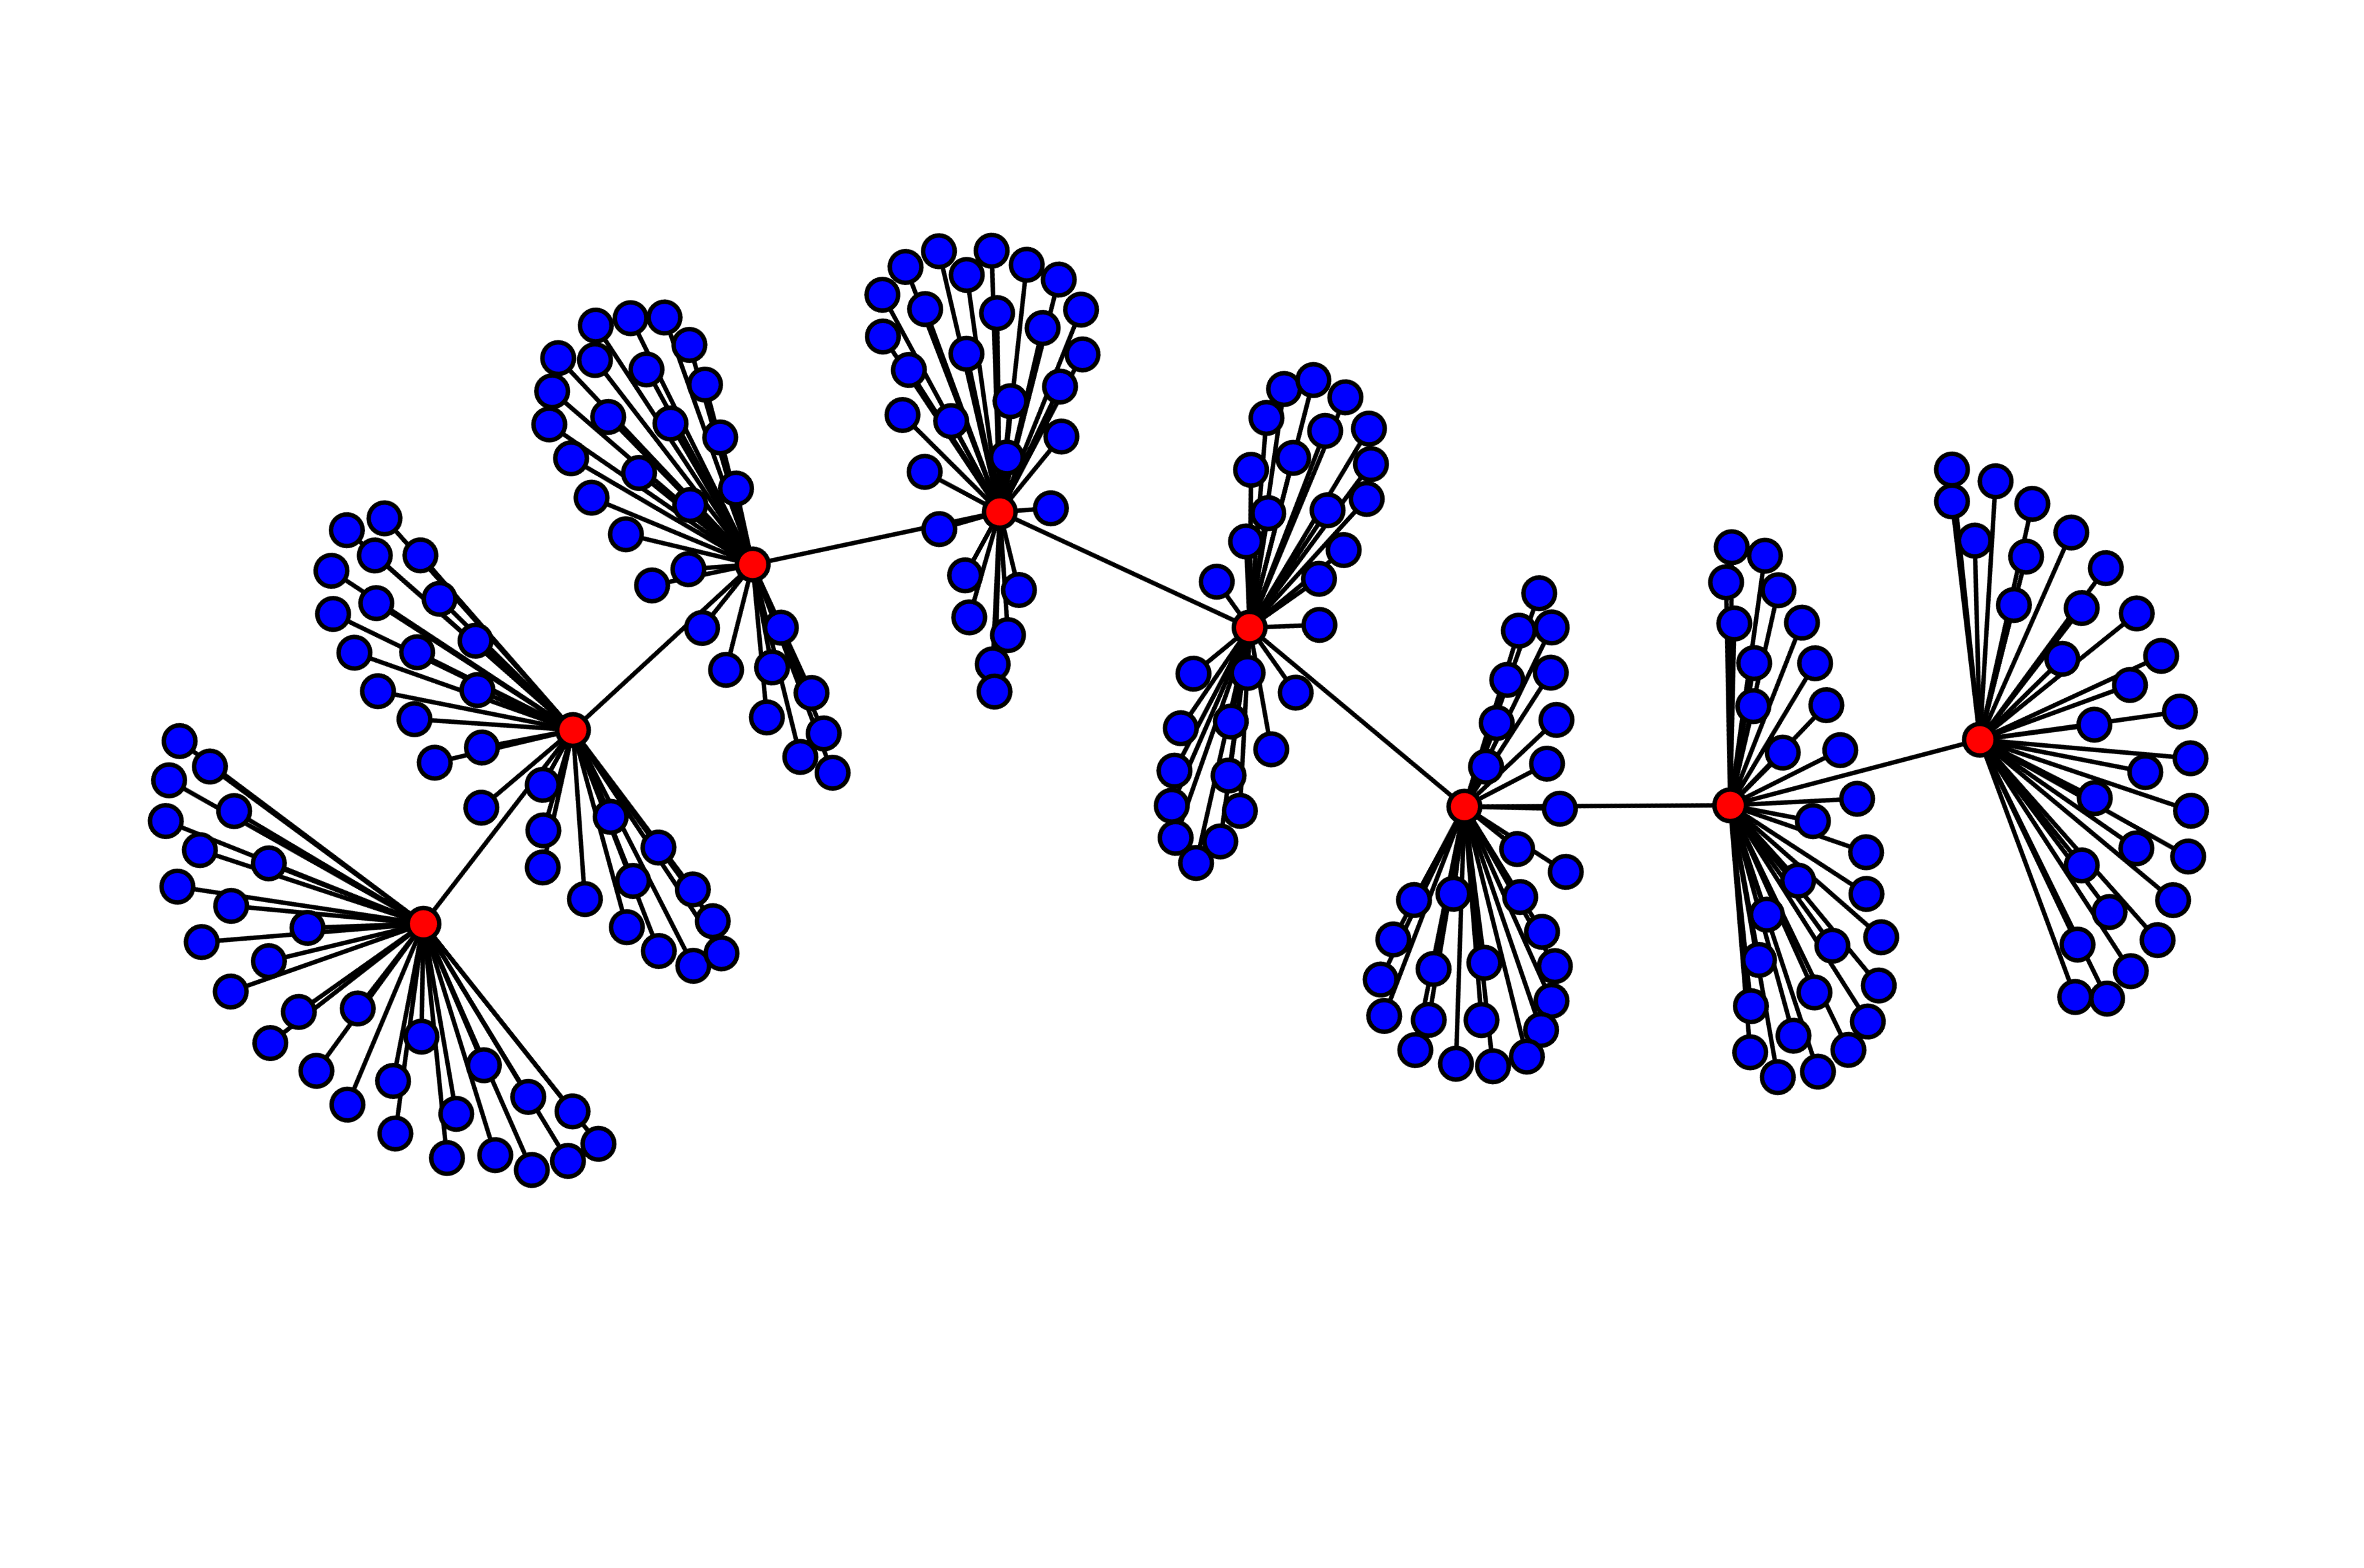
\includegraphics[width=\textwidth]{img/full-graph}
    \caption{Grafo representando uma rede com 248 entidades}
    \label{fig:full-graph}
\end{figure}
\break
Um experimento foi executado na rede Ipê para mostrar as alterações na 
representação do grafo.

No instante inicial, o controlador é iniciado.
Cada comutador estabelece uma conexão segura com o controlador.
Nesse momento, todos os vértices comutadores são adicionados ao grafo.
No segundo instante, para apenas uma subrede, representando uma unidade 
federativa dentro da rede Ipê, foi simulado tráfego entre seus computadores.
Para cada computador, uma sondagem de todos os outros computadores dessa
subrede foi feita através do utilitário \emph{ping}.
Assim, todas as máquinas dessa subrede foram identificadas pelo controlador
e adicionadas ao grafo representando a rede.
No terceiro instante, outra subrede foi escolhida e a mesma simulação de 
tráfego foi executada.
O mesmo procedimento foi repetido até que todas as 27 subredes da rede Ipê
fossem computadas pelo grafo.

A figura \ref{fig:full-graph-ipe} apresenta a execução desse experimento 
cronologicamente.
Cada número representa a quantidade de redes computadas pelo grafo no instante
da execução do experimento. 
Uma rede com 563 computadores e 27 comutadores (\emph{switches}) é mostrada
na imagem Final da figura \ref{fig:full-graph-ipe} representando toda a rede
Ipê.
No total o grafo computou 590 vértices.

\begin{figure}[htb!]
    \centering
    \label{fig:full-graph-ipe}
    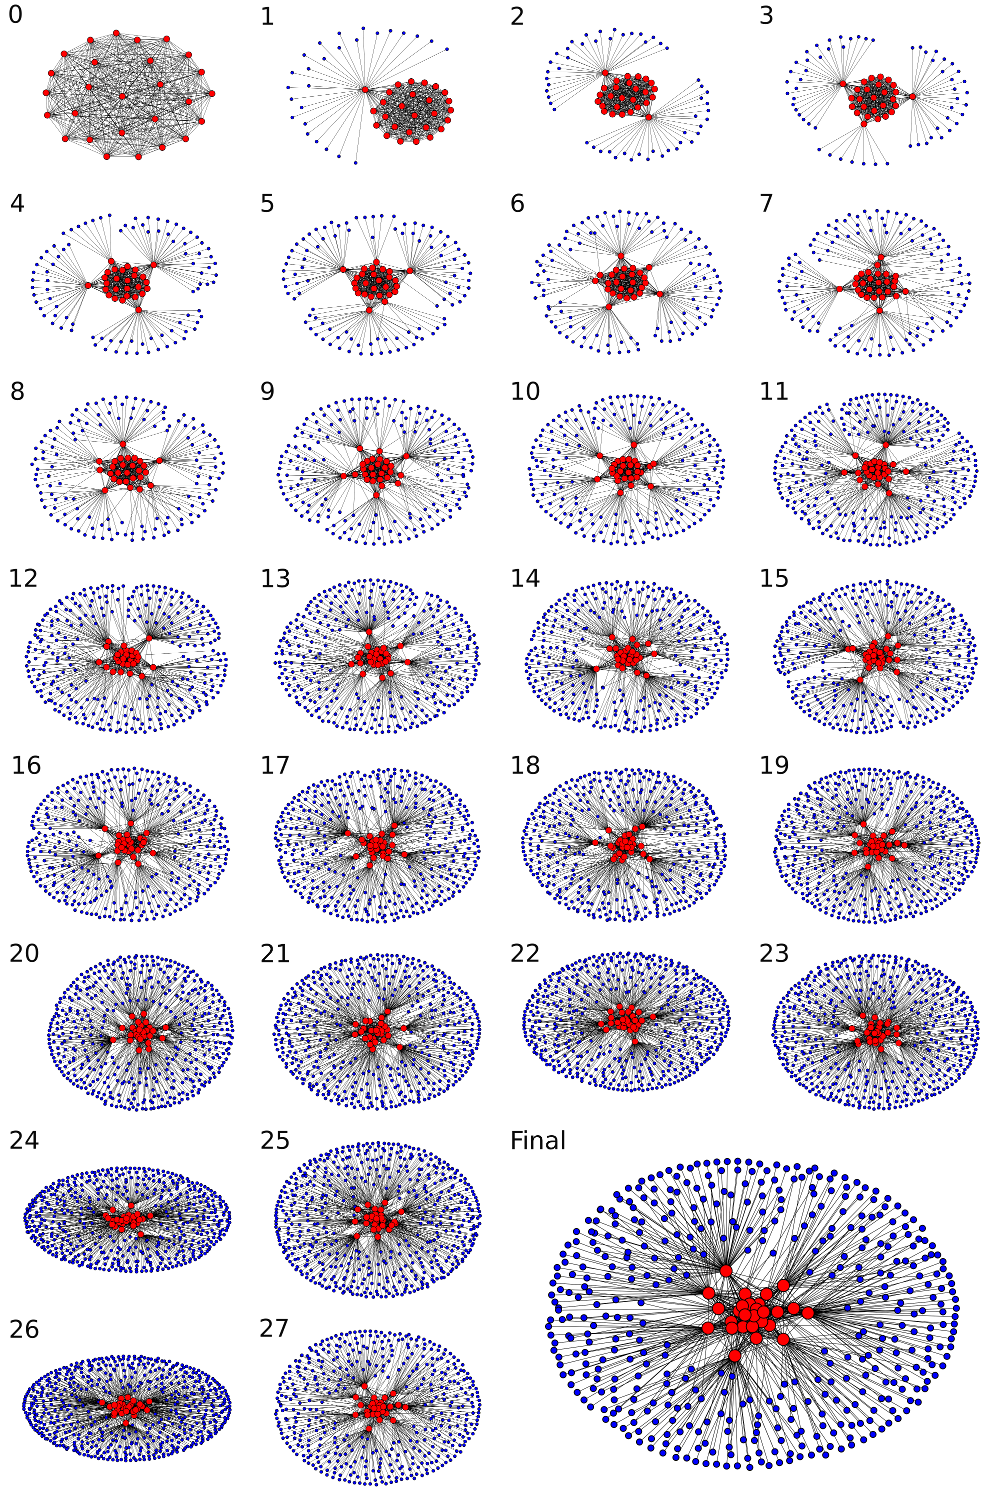
\includegraphics[scale=0.395]{img/full-graph-ipe}
    \caption{Representação da rede Ipê à medida que os computadores de cada
    subrede são identificados}
\end{figure}


\section{Identificação de tráfego}

Para computar o tráfego (TCP) em uma rede simples foi executado o programa 
\emph{iperf} como servidor no \emph{host} 'Host 0a'.
A topologia dessa rede é composta por dois comutadores interligados.
Cada comutador possui três computadores em cada subrede.
O \emph{host} 'Host 1e' conecta-se como cliente. 

Conformo pode ser notado na figura \ref{fig:iperf}, o tráfego 
em bytes na arestas desses \emph{hosts} é superior ao demais \emph{hosts}.
No momento em que foram lidos os contadores \emph{OpenFlow} e computados
os pesos das arestas, obteve-se um tráfego de 55894 bytes através do caminho
entre os dois \emph{hosts} citados.
Os valores apresentados para os demais \emph{hosts} (41 bytes) são referentes
ao tráfego ARP PING disseminado pelo módulo \emph{host\_tracker}

\begin{figure}[h!]
    \centering
    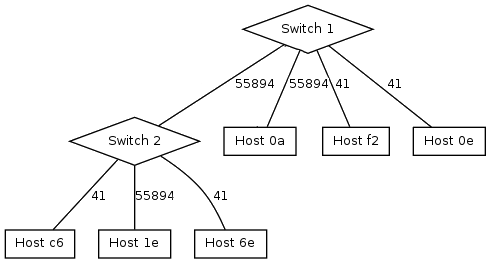
\includegraphics[scale=0.8]{img/graph-iperf}
    \caption{Tráfego TCP (em bytes) entre os hosts ’Host 1e’ e ’Host 0a’}
    \label{fig:iperf}
\end{figure}

\section{Avaliação do Controlador}

O consumo da unidade central de processamento (CPU) no processo do controlador,
no sistema operacional, assim como a utilização de memória e taxa de escrita 
em disco foram medidos através da biblioteca utilitária \emph{sysstat} 
\citep{sebastien2015sysstat}.

Um experimento variando o número de computadores na rede permitiu coletar 
as métricas citadas acima.
Coletou-se durante 30 segundos a utilização da CPU do processo do controlador,
do sistema operacional, a utilização de memória e a taxa de escrita em disco
em cada interação da execuçao do experimento.
A cada iteração do experimento, 50 novos computadores foram adicionados a rede.
Ou seja, o experimento começou com 50 computadores e terminou com 550.

\subsection{Consumo de processador no processo do controlador}


Conforme pode ser visto na figura \ref{fig:usr-cpu-growth}, considerando a 
variação das medições feitas no experimento, o crescimento da curva de 
utilização de CPU mostra-se logarítmica.
Apesar desse comportamento para o processo do controlador, nota-se que o 
consumo, analisando todo o sistema, é linear.
Esses resultados são apresentados na próxima seção. 
O comportamento logarítmo mostra que, apesar do aumento do número de
computadores na rede, o processo do controlador não gerou exaustão na CPU 
alocada para o processo ao longo do experimento.
À medida que a rede cresce, a utilização da CPU escalonada ao processo do 
controlador, cresce na mesma proporção.

\begin{figure}[htb!]
    \centering
    \label{fig:usr-cpu-growth}
    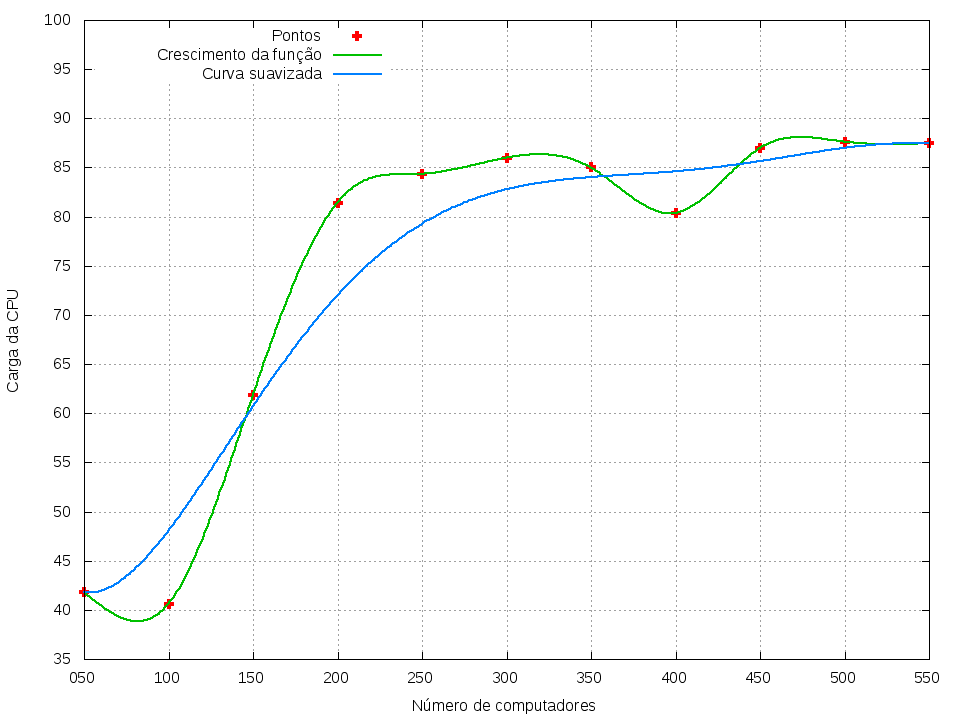
\includegraphics[width=\linewidth]{img/usr-cpu-growth.png}
    \caption{Variação do consumo médio de CPU no processo do controlador à 
    medida que a rede cresce}
\end{figure}

Uma regressão linear foi computada em cima da amostra coletada da utilização 
de CPU pelo processo do controlador.
A figura \ref{fig:scatter-usr-cpu} apresenta os resultados dessa computação.
É possível notar o crescimento da utilização de CPU à medida que a rede cresce.
A dispersão dos valores no início da amostragem estão mais próximos de 0. 
Ou seja, a rede com poucos computadores demandou baixo processamento. 
Já nos instantes finais, há mais pontos amostrados próximos a 100\% da 
utilização de CPU, o que mostra o estress do processador com uma rede maior.

\begin{figure}[!htb]
    \centering
    \label{fig:scatter-usr-cpu}
    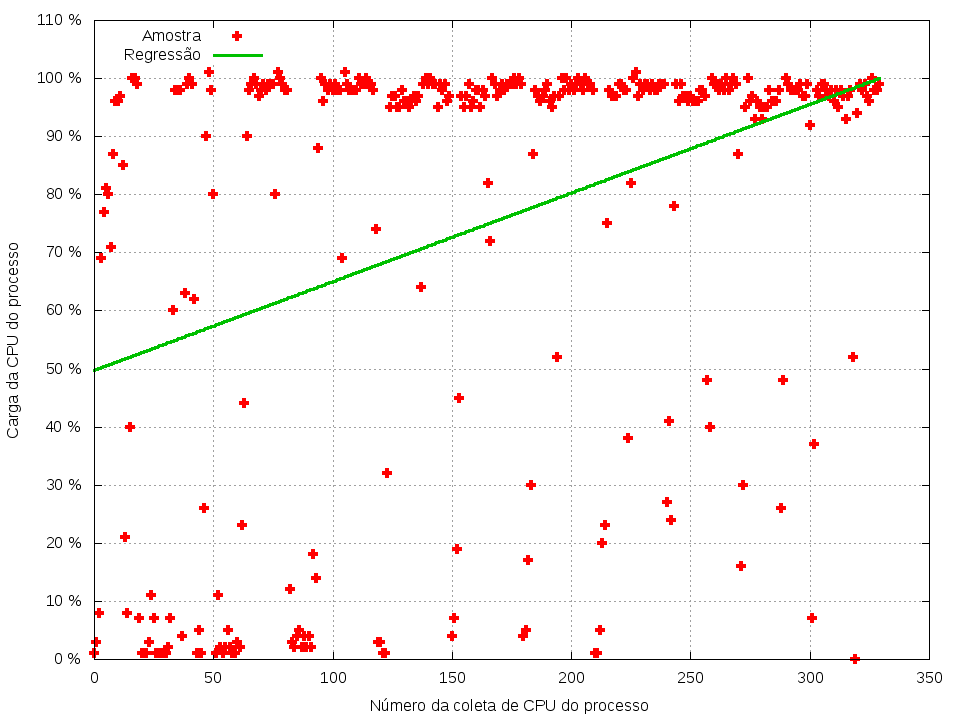
\includegraphics[width=\linewidth]{img/scatter-usr-cpu}
    \caption{Regressão linear da utilização de CPU do processo do controlador
    em função do número de coletas de CPU realizadas à medida que a rede 
    crescia}
\end{figure}

A reta representada pela regressão mostra o quão crescente é a utilização de 
CPU pelo processo à medida que a rede cresce.


\subsection{Consumo do controlador em relação ao sistema operacional}

Para computar um rede com 550 computadores o controlador utilizou 10\% da 
CPU do sistema operacional.
Como pode ser visto na figura \ref{fig:sys-cpu-growth} o crescimento da 
função de utilização de CPU do sistema é praticamente linear.
À medida que a rede cresce, os processadores do computador do controlador 
aumentam sua carga.

\begin{figure}[!htb]
    \centering
    \label{fig:sys-cpu-growth}
    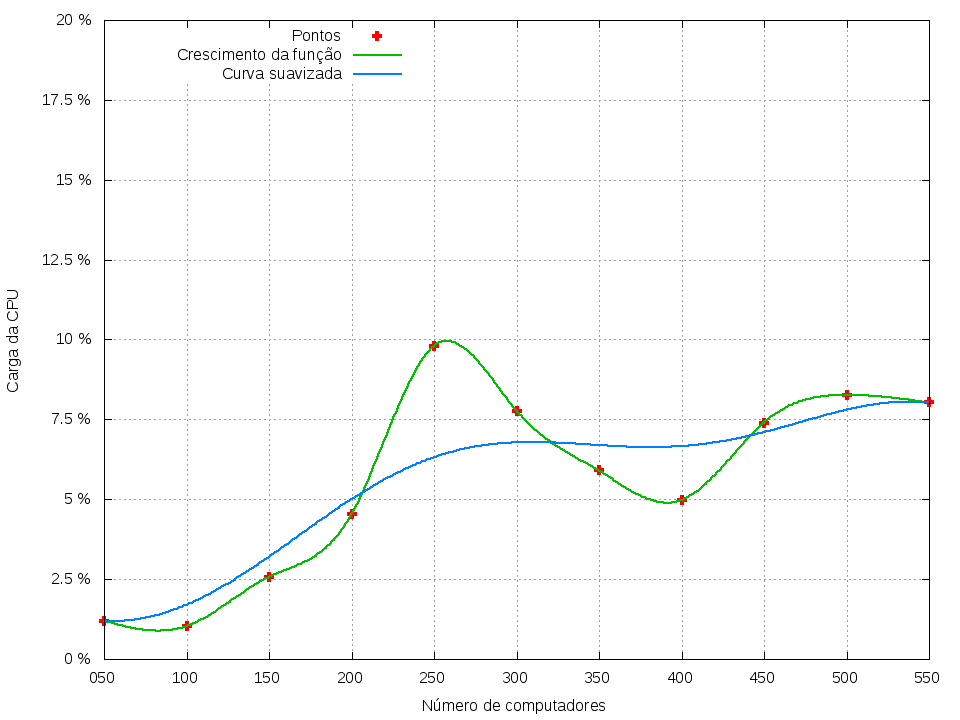
\includegraphics[width=\linewidth]{img/sys-cpu-growth}
    \caption{Crescimento da função de utilização da CPU do sistema operacional
    em função do crescimento de computadores na rede}
\end{figure}

O controlador POX é escrito na linguagem de programação \emph{Python}.
Cada nova entidade (computador ou comutador) ao ser detectado pelo controlador
recebe um identificador único.
Essas entidades são armazenadas em um dicionário \emph{Python}.
O dicionário é uma estrutura de dados primitiva da linguagem que implementa
uma tabela \emph{hash} \citep{maurer1975hash}.
Em função disso, para a computação do experimento temos que a complexidade 
de tempo é na ordem de $O(n)$ conforme mostrado a seguir.

As operações de adição, remoção e busca em tabelas \emph{hash} tem, no 
caso médio, custo constante na ordem de $O(1)$.
Assim, considerando-se $n$ o número de vértices, temos que para cada 
vértice do grafo o custo para inserí-lo durante o experimento é $O(1)$.
A complexidade de tempo do experimento, à medida que a rede cresce, é na 
ordem de $O(n)$.

Uma regressão linear foi computada da amostra coletada da carga de \emph{CPU}
do sistema operacional durante o experimento. 
A figura \ref{fig:scatter-sys-cpu} apresenta o resultado da regressão.

\begin{figure}[!htb]
    \centering
    \label{fig:scatter-sys-cpu}
    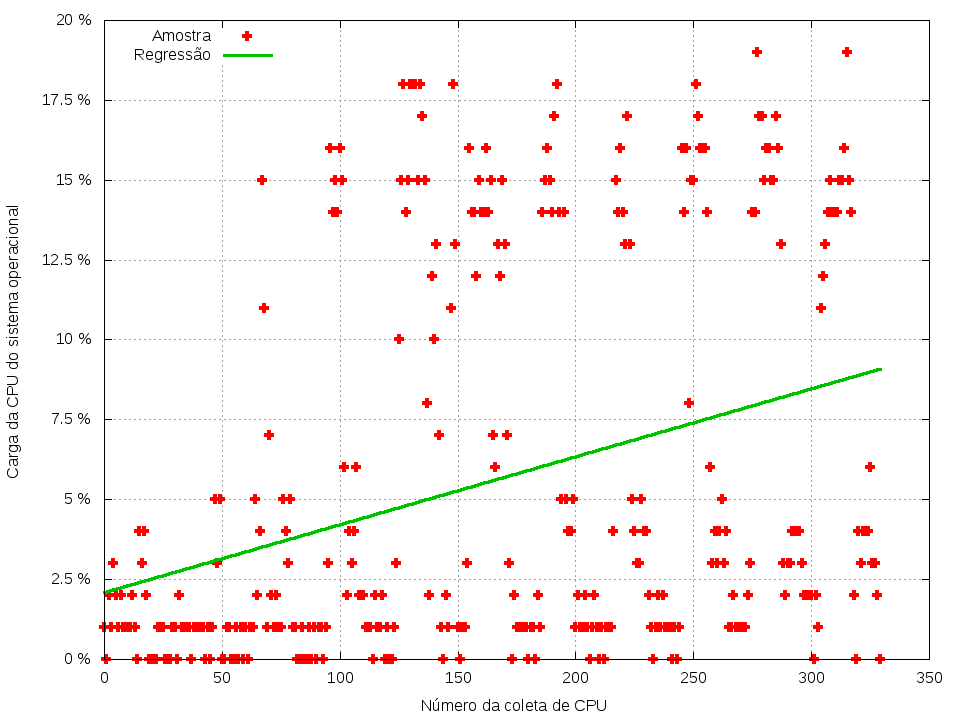
\includegraphics[width=\linewidth]{img/scatter-sys-cpu}
    \caption{Regressão linear sobre a carga de CPU do sistema operacional}
\end{figure}


\subsection{Consumo de memória}

A figura \ref{fig:memory-usage-growth} apresenta o crescimento da utilização
de memória à medida que a rede cresce. 
O computador do controlador possui 8 \emph{Gigabytes} de memória RAN 
(\emph{random access memory}). 
O consumo de memória pelo controlador durante o experimento variou de 2\% a 4\%
da memória global do sistema operacional.

O módulo \emph{Graph} adiciona vértices para cada computador e comutador 
identificados na rede.
Cada vértice é um objeto da classe \emph{Vertex}.
Esse objeto contém a referência para objetos das classes \emph{Host} e 
\emph{Switch} da entidade (computador ou comutador) que é representada pelo
vértice.
Assim, à medida que vértices são adicionados à rede, novos objetos são 
criados.
As arestas são objetos da classe \emph{Edge} e guardam referências para 
os objetos dos vértices que compõem a aresta.

\break
\begin{figure}[!htb]
    \centering
    \label{fig:memory-usage-growth}
    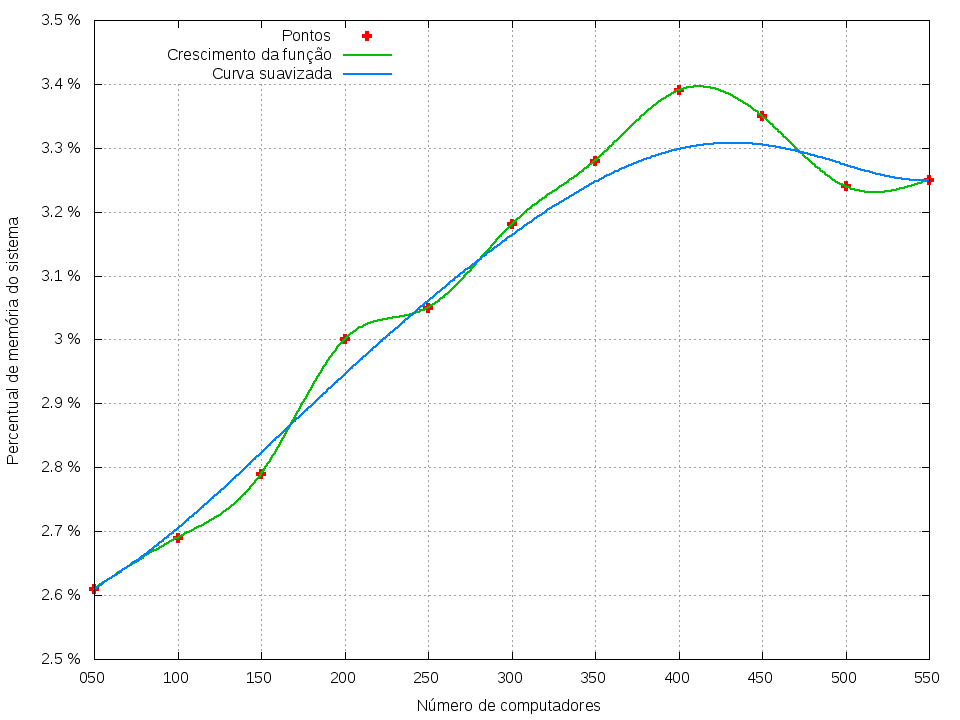
\includegraphics[width=\linewidth]{img/memory-usage-growth}
    \caption{Crescimento do percentual de utilização de memória pelo
    controlador à medida que o número de computadores na rede aumenta}
\end{figure}

Em função disso, assumiu-se que: Um objeto \emph{Vertex} ocupa na memória um 
espaço de endereçamento de tamanho $x$. 
E um objeto \emph{Edge} ocupa $y$.
Considerando-se $n$ o número de vértices e $m$ o número de arestas do grafo,
temos que a função que representa a utilização de memória (complexidade de 
espaço) é $nx + my$.
Ou seja, o número de vértices no grafo multiplicado pelo tamanho de um 
objeto de vértice na memória somado ao número de arestas do grafo 
multiplicado pelo tamanho de um objeto de aresta na memória.


A função de complexidade de espaço $nx + my$ mostra que o crescimento de 
utilização de memória do computador é dada em função do aumento de vértices
e arestas na rede.
No experimento executado, o número de vértices (coeficiente $n$) cresceu 
linearmente.
A regressão linear computada mostra o crescimento na utilização de memória 
pelo controlador à medida que mais computadores foram inseridos na rede ao 
longo da amostragem.
A figura \ref{fig:scatter-memory-usage} apresenta o resultado dessa 
computação.

\begin{figure}[!htb]
    \centering
    \label{fig:scatter-memory-usage}
    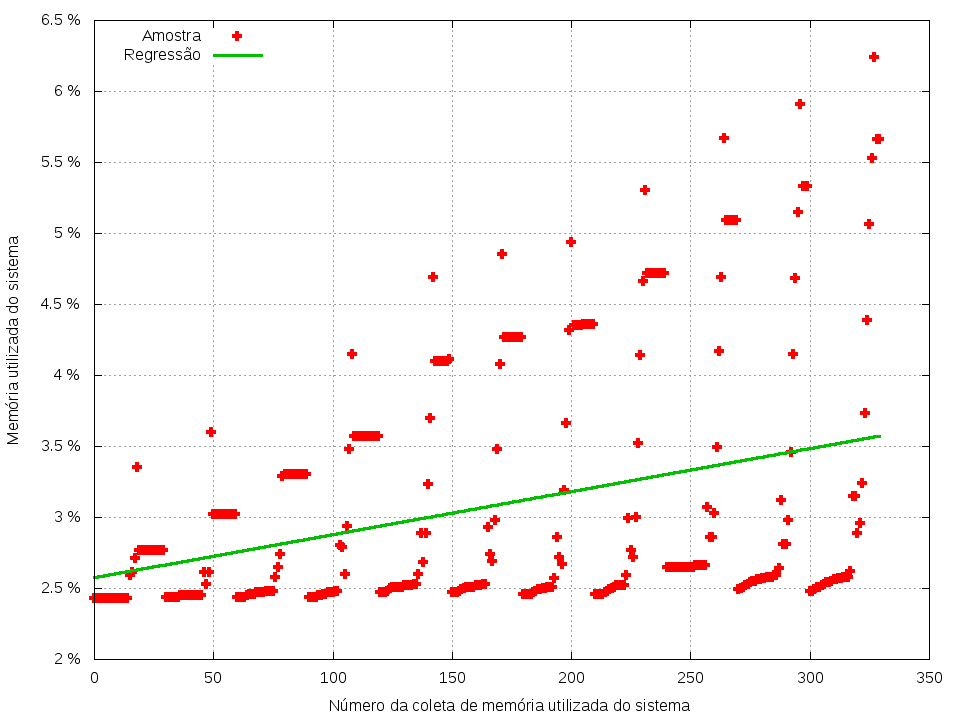
\includegraphics[width=\linewidth]{img/scatter-memory-usage}
    \caption{Regressão linear da amostra do consumo de memória do sistema
    à medida que rede cresce}
\end{figure}


\subsection{Taxa de escrita em memória secundária}

O módulo \emph{Graph} periodicamente salva uma imagem em memória secundária
com a visualização do grafo.
Durante o experimento de avaliação do controlador foi coletada a taxa de
escrita em disco à medida que a rede crescia. 

Em média, a taxa de escrita foi de 2 \emph{Megabytes} ao longo de cada 
iteração do experimento.
Para o experimento, uma imagem era gravada a cada 25 segundos.
Em cada iteração, mais vértices haviam no grafo, logo, mais objetos a serem 
mapeados na imagem. 

\break

Na figura \ref{fig:writing-rate-growth} é possível ver o crescimento na 
taxa de escrita em memória secundária à medida que a rede crescia.
Os pontos em vermelho representam os valores máximos de escrita coletados 
em cada iteração do experimento.
Uma interpolação passando por todos os pontos é dada pela curva de coloração
verde.
Uma suavização da curva de interpolação é traçada na cor azul mostrando 
o crescimento da taxa de escrita à medida que novos vértices vão sendo criados
durante as iterações do experimento.

\begin{figure}[!htb]
    \centering
    \label{fig:writing-rate-growth}
    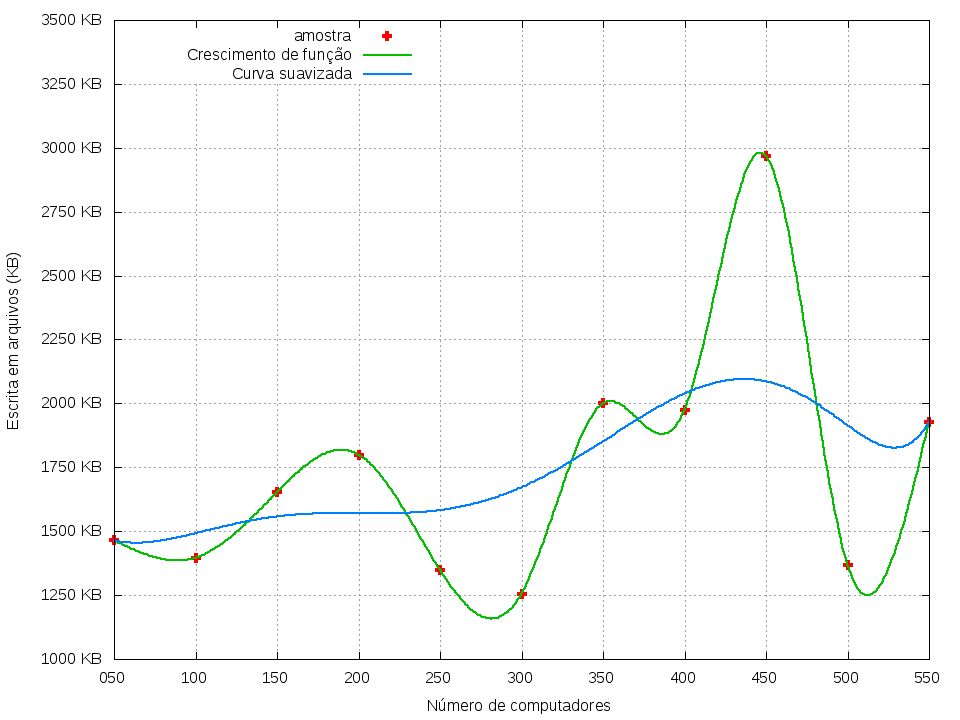
\includegraphics[width=\linewidth]{img/writing-rate-growth}
    \caption{Taxa de escrita em memória secundária à medida que a rede cresce}
\end{figure}

Uma regressão linear foi computada na amostra coletada das taxas de escrita
em memória secundária ao longo do experimento.
A figura \ref{fig:scatter-writing-rate} apresenta o resultado dessa regressão
mostrando o crescimento e a correlação entre os valores amostrados.

\begin{figure}[!htb]
    \centering
    \label{fig:scatter-writing-rate}
    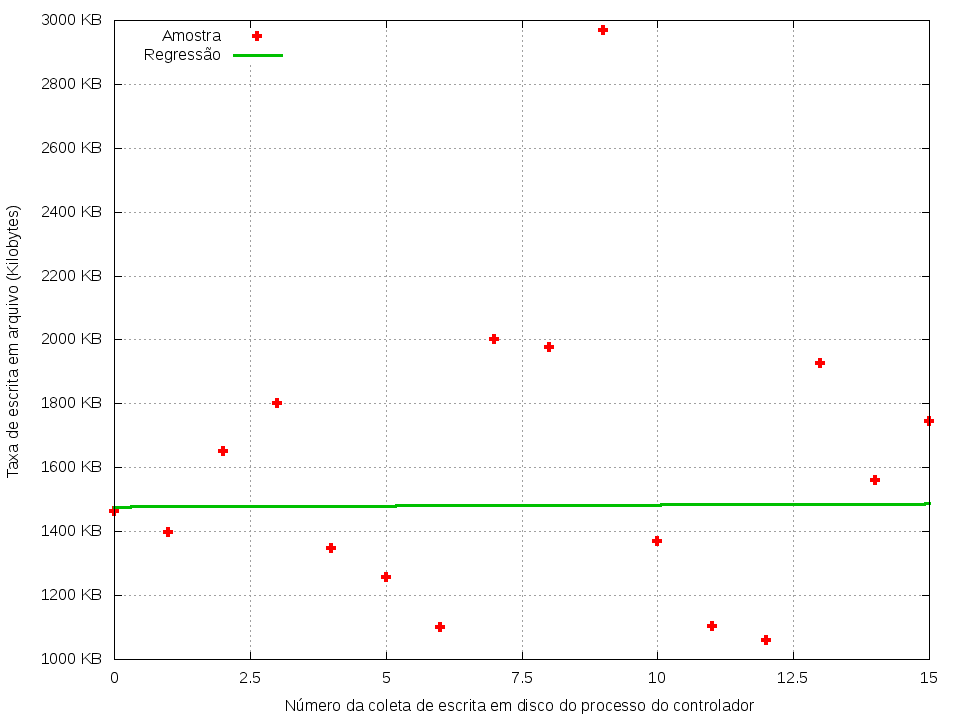
\includegraphics[width=\linewidth]{img/scatter-writing-rate}
    \caption{Regressão linear dos valores coletados da taxa de escrita em 
    memória secundária}
\end{figure}

\break
\section{Avaliação do módulo \emph{host\_tracker}}

O módulo \emph{host\_tracker} periodicamente envia pacotes \emph{APPPings} de
sondagem aos computadores da rede. 
Esta seção avalia o impacto e comportamento desse módulo em relação a rede e 
a solução.

Primeiramente é avaliada a largura de banda da rede e o impacto da sondagem 
de computadores nessa propriedade.
Em seguida a proporção de pacotes manipulados pelo controlador é comparada
em relação a quantidade de pacotes de sondagem.

\subsection{Avaliação de largura de banda}

Para medir a largura de banda foi utilizada a ferramenta de linha comando
\emph{iperf}.
A rede Ipê foi simulada com o conjunto completo de computadores.
6 pares de clientes e servidores \emph{iperf} foram executados durante 300 
segundos.
Cada par de cliente e servidor foi instanciado em máquinas virtuais 
diferentes e físicamente separadas.

\begin{table}[h!]
    \centering
    \begin{tabular}{ | l | l | l | l |}
    \hline
    \textbf{Teste} & \textbf{pingLim} & \textbf{entryMove} &
    \textbf{arpReply} \\ 
    \hline
    \hline Teste 0 & 5 & 50 & 5 \\ 
    \hline Teste 1 & 4 & 40 & 4 \\ 
    \hline Teste 2 & 3 & 30 & 3 \\ 
    \hline Teste 3 & 2 & 20 & 2 \\
    \hline Teste 4 & 1 & 10 & 1 \\
    \hline
    \end{tabular}
    \caption{Tabela com a relação de parâmetros por teste}
    \label{tbl:host_tracker-experiment}
\end{table}


Foram executados 5 baterias de testes.
Cada teste variou 3 parâmetro do módulo \emph{host\_tracker}.
O parâmetro \emph{pingLim} representa a quantidade de pacotes de sondagem 
necessários para considerar que um computador está inativo.
O parâmetro \emph{entryMove} é o tempo até que uma entrada do dicionário de 
endereços MAC seja alterado.
E o parâmetro \emph{arpReply} é o tempo a ser esperado pela resposta ARP até
que uma nova tentativa de sondagem seja enviada.
A tabela \ref{tbl:host_tracker-experiment} mostra de maneira resumida os 
experimentos executados.

\begin{figure}[!htb]
    \centering
    \label{fig:host_tracker-bandwidth}
    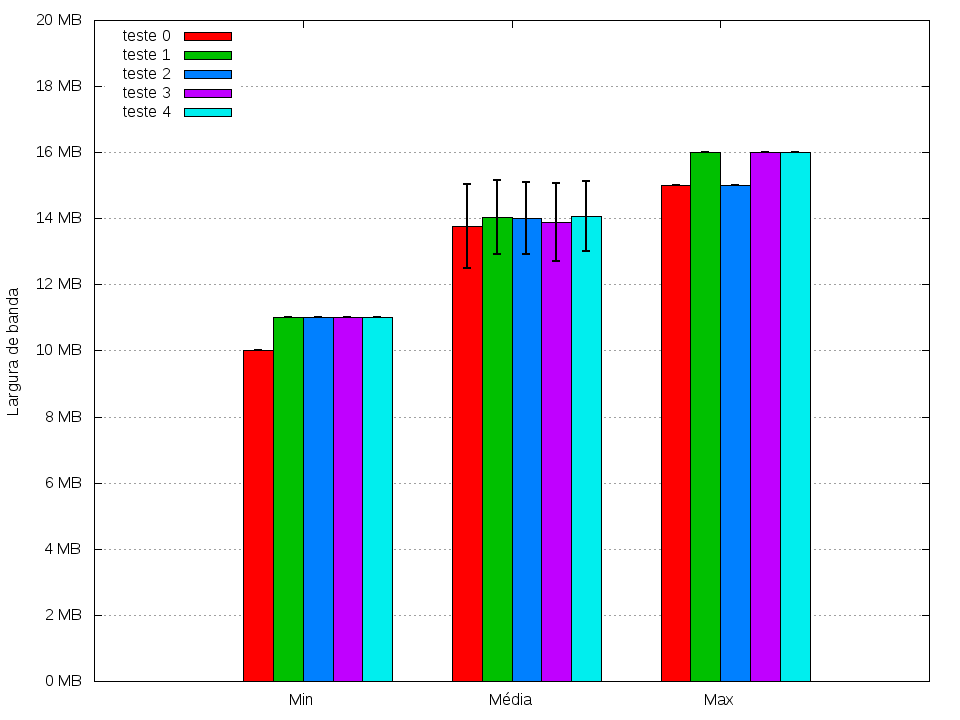
\includegraphics[width=\linewidth]{img/host_tracker-bandwidth}
    \caption{Largura de banda mínima, média com intervalo de confiança e máxima
    coletada da execução de cada teste do experimento}
\end{figure}

Para cada teste, durante 300 segundos, a cada 5 segundos a largura de banda
foi coletada.
A figura \ref{fig:host_tracker-bandwidth} mostra os valores mínimos, médio 
com intervalo de confiança e máximo da largura de banda coletada nos testes.

Como existiam 6 pares de clientes e servidores, a largura de banda é 
dividida entre esses computadores.
A média foi computada do somatório da largura de banda computada por cada 
par de cliente e servidor.

Conforme visto na tabela \ref{tbl:host_tracker-experiment} do Teste 0 ao 
Teste 4 os parâmetros avaliados foram decrementados. 
Em função disso, à medida que os testes foram executados nessa ordem, 
o intervalo de sondagem, o tempo de expiração e o tempo de aguardo por 
resposta reduziram. 
Essa redução faz com que a cada iteração de testes mais pacotes de sondagem
fossem disseminados na rede.
A figura \ref{fig:host_tracker-bandwidth} mostra que, apesar do aumento de 
pacotes de sondagem, a largura de banda média da rede não sofreu impacto 
considerável.
A figura \ref{fig:host_tracker-bandwidth-growth} apresenta a curva de 
interpolação entre os pontos representando a largura de banda média em cada 
teste do experimento.

\begin{figure}[!htb]
    \centering
    \label{fig:host_tracker-bandwidth-growth}
    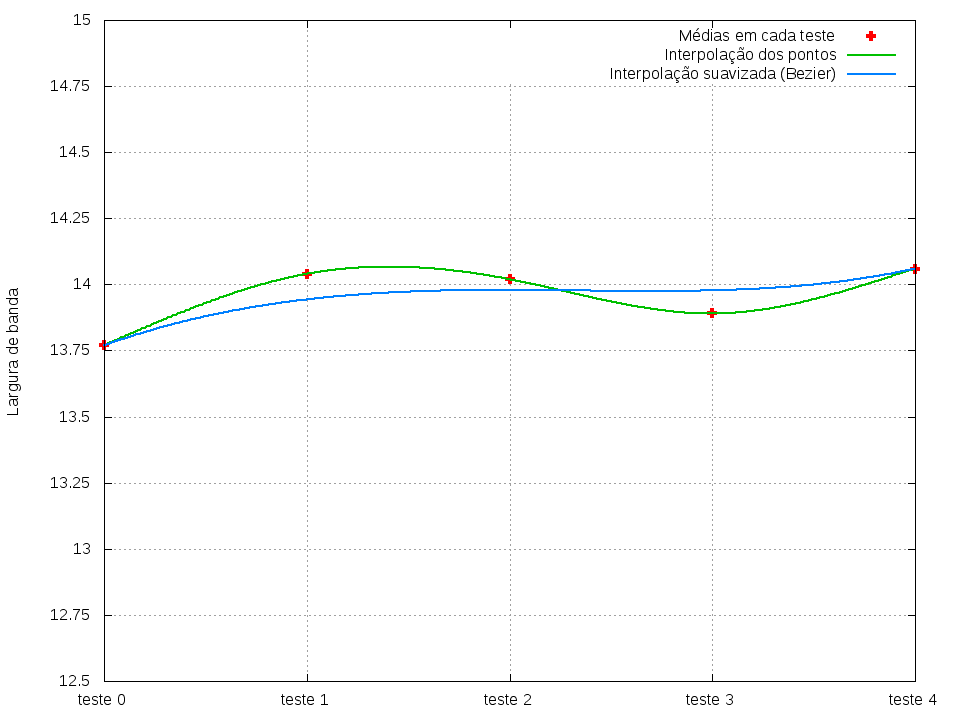
\includegraphics[width=\linewidth]{img/host_tracker-bandwidth-growth}
    \caption{Curva de interpolação das médias das larguras de banda medidas 
    em teste do experimento}
\end{figure}

\subsection{Avaliação do número de pacotes}

Essa subseção avalia a quantidade de pacotes de sondagem disparadas pelo 
módulo \emph{host\_tracker} à medida que mais computadores estão presentes
na rede.
São avaliados também, a quantidade de pacotes de entrada (\emph{PacketIn}) 
que o controlador lida à medida que a rede cresce.

O experimento começou com 50 computadores na rede.
Em cada iteração, novos 50 computadores foram adicionados à rede.
Ao final, a rede Ipê simulada, possuía 550 computadores.
Para computar o número de pacotes de sondagem foi adicionado um contador 
na funçao que envia esses pacotes.
A figura \ref{fig:npings} mostra o gráfico resultante dos valores computados
dos número de pacotes de sondagem enviados à medida que mais computadores 
estavam presentes na rede.

\begin{figure}[!htb]
    \centering
    \label{fig:npings}
    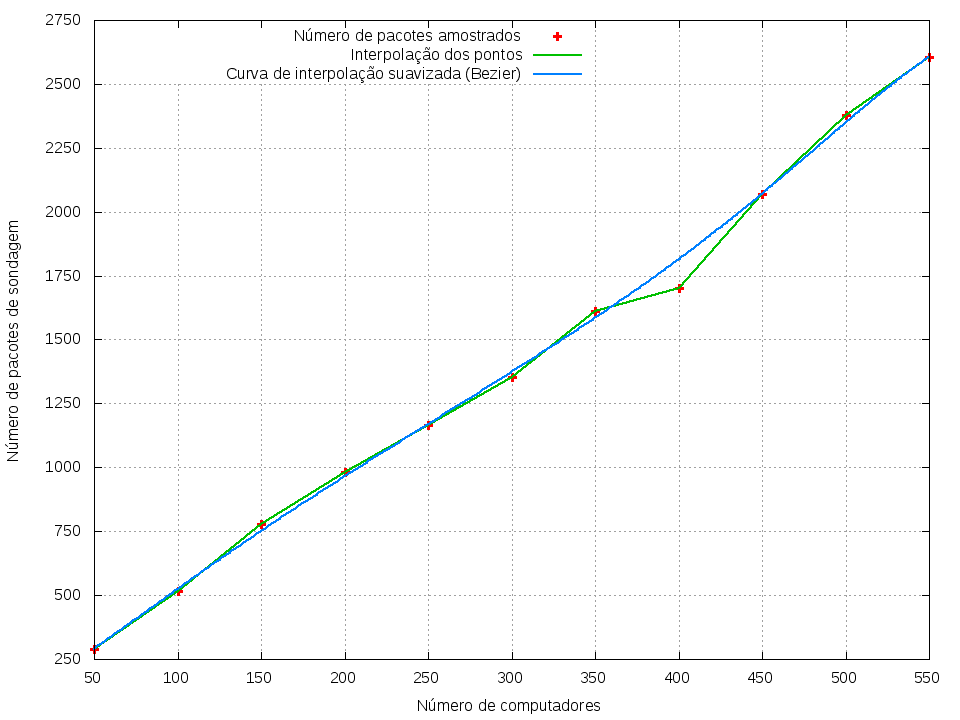
\includegraphics[width=\linewidth]{img/npings}
    \caption{Crescimento do número de pacotes de sondagens encaminhados 
        à medida que a rede crescia}
\end{figure}

O aumento do número de pacotes apresentou um crescimento linear.
Ou seja, à medida que mais computadores entram na rede, o número de pacotes
cresce na mesma proporção.
Para esse experimento, foi calculada a diferença da quantidade de pacotes da
iteração posterior com a iteração anterior.
Assim, é possível saber quantos pacotes variaram a cada iteração do 
experimento.
Esse resultado é apresentado na figura \ref{fig:npings-stats}. 

Em média, 200 a 250 pacotes a mais foram disparados a cada iteração. 
O experimento durou, para cada iteração, dois minutos. 
Considerando esse intervalo de tempo e a média de pacotes enviados, pode-se 
dizer que aproximadamente 5 pacotes foram enviados para cada computador 
identificado pelo grafo.
Levando em conta a média de 250 pacotes por iteração e que cada iteração 
adiciona 50 novos computadores, temos que a razão desses valores mostra 
que, para cada computador, durante dois minutos foram enviados 5 pacotes 
de sondagem.

\begin{figure}[!htb]
    \centering
    \label{fig:npings-stats}
    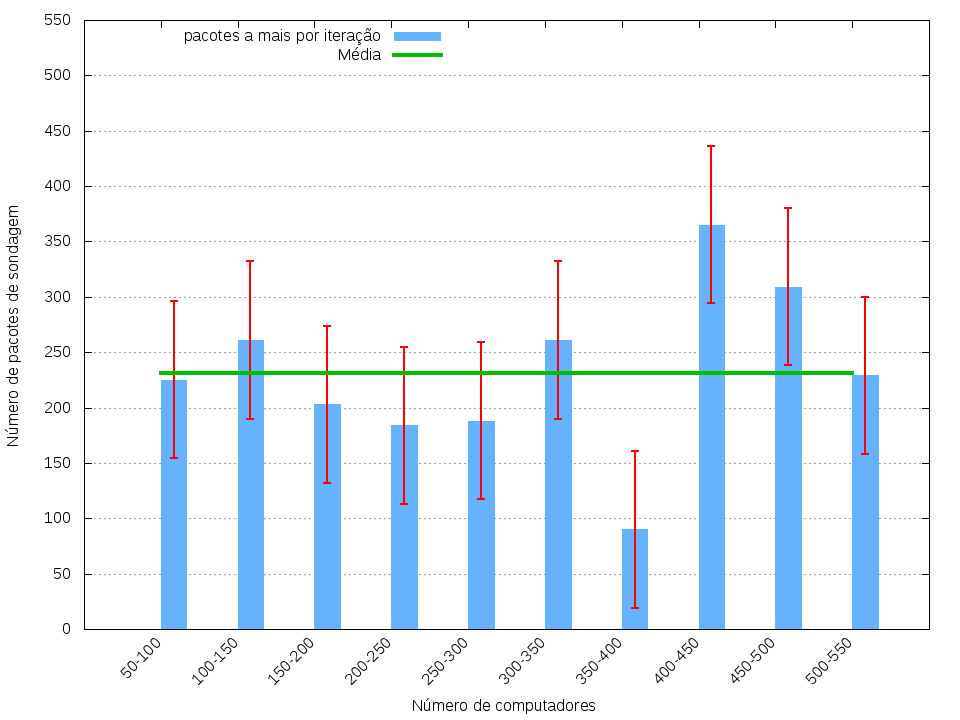
\includegraphics[width=\linewidth]{img/npings-stats}
    \caption{Diferença da quantidade de pacotes de sondagem enviados entre 
    cada par de iterações do experimento}
\end{figure}

O número de pacotes de entrada foi contabilizado contando as chamadas do 
evento \emph{PacketIn} no controlador.
Foram medidos quantos pacotes de entrada o controlador manipulava a cada 
iteração do experimento.

A figura \ref{fig:packets-in} mostra o crescimento no número de pacotes ao 
longo do experimento. 
Assim como o número de pacotes de sondagem, o número de pacotes 
(\emph{PacketIn}) cresce linearmente.
Ou seja, à medida que mais computares estão na rede, o volume de pacotes de 
entrada cresce proporcionalmente.

\begin{figure}[!htb]
    \centering
    \label{fig:packets-in}
    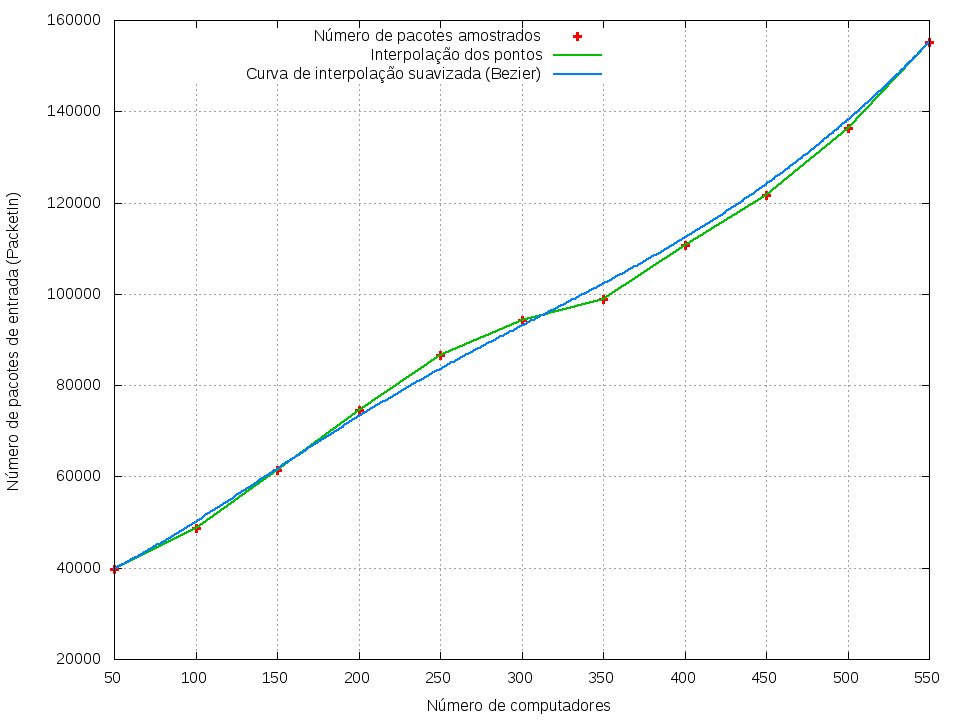
\includegraphics[width=\linewidth]{img/packets-in}
    \caption{Número de pacotes de entrada (\emph{PacketIn}) manipuladas pelo
    controlador em cada iteraçao do experimento}
\end{figure}


Para o experimento da contagem do número de pacotes de entrada no controlador
foram computadas as diferenças entre os experimentos posteriores e os
anteriores.
Em média doze mil pacotes de entrada foram manipulados a mais em cada 
iteração do experimento.

A figura \ref{fig:packets-in-stats} mostra os resultados desse experimento.
A linhas verticais vermelhas apresentam o intervalo de confiança dos valores
amostrados das diferenças. 
O erro padrão baixo prova o comportamento mostrado na figura 
\ref{fig:packets-in} sobre o crescimento linear no número de pacotes de 
entrada.

Considerando o intervalo de tempo de dois minutos de execução do experimento e 
que, a cada iteração cinquenta novos computadores foram adicionados, 
tem-se que a razão da média pelo número de computadores por iteração é igual 
a 250 pacotes. 
O controlador lida com pacotes que nem sempre são originados de computadores.
Assim, esse valor calculado é apenas uma aproximação do número de pacotes 
que o controlador manipula em função do número de computadores.

\begin{figure}[!htb]
    \centering
    \label{fig:packets-in-stats}
    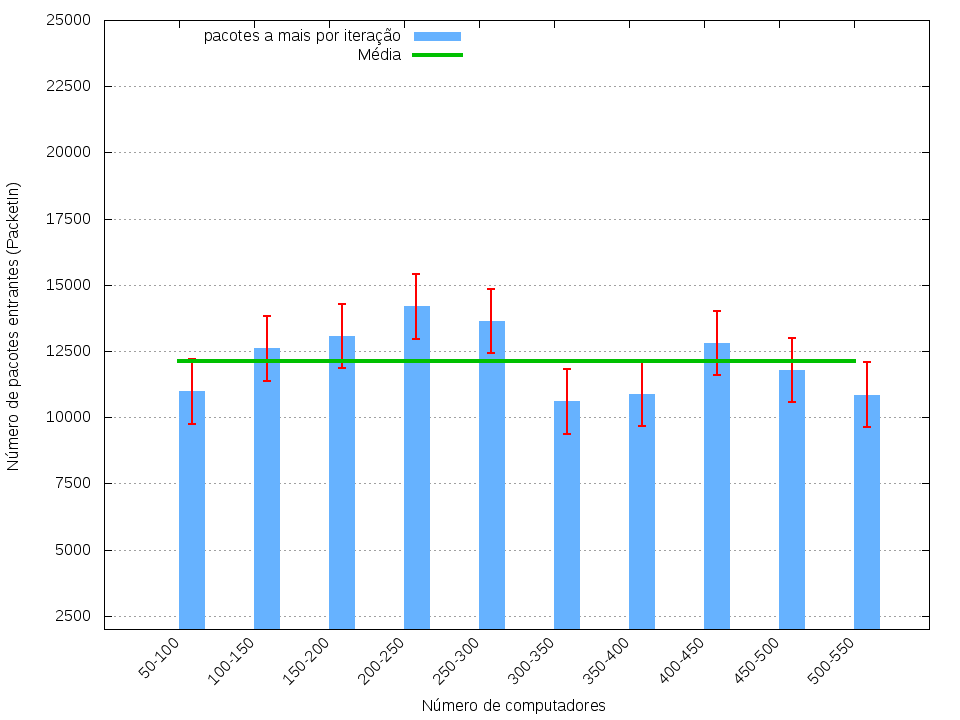
\includegraphics[width=\linewidth]{img/packets-in-stats}
    \caption{Diferença da quantidade de pacotes de entrada (\emph{PacketIn})
    manipuladas no controlador entre cada par de iterações do experimento}
\end{figure}

\subsection{Comparação dos números de pacotes}

Essa subseção compara o número de pacotes de sondagem com o número de pacotes
de entrada que o controlador lida.
A comparação é feita em quantidade e em percentual.
A seguir serão apresentados os resultados dessa avaliação.

A comparação do número de pacotes é mostrada na figura
\ref{fig:npings-x-packets-in}.
Os valores nas coordenadas $y$ (ordenadas) estão em escala exponencial, o que 
facilita a visualização da diferença entre o número de pacotes de entrada
(\emph{PacketIn}) e pacotes de sondagem.

Com a rede Ipê simulada completa foram enviados, no máximo, quase $3$ mil 
pacotes de sondagem e quase $150.000$ pacotes de entrada manipulados pelo 
controlador.
\break
\begin{figure}[!htb]
    \centering
    \label{fig:npings-x-packets-in}
    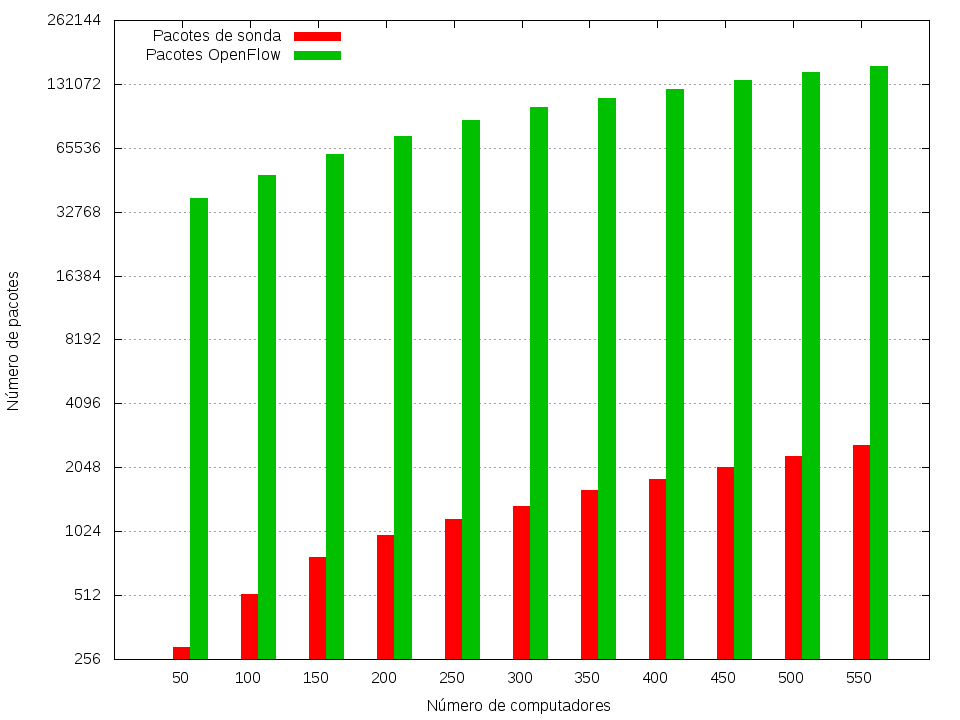
\includegraphics[width=\linewidth]{img/npings-x-packets-in}
    \caption{Comparação do número de pacotes de sondagem e de entrada 
    manipulados pelo controlador}
\end{figure}

O total de pacotes manipulados pelo controlador é representado pela soma 
do número total de pacotes de sondagem com o número total de pacotes de 
entrada (\emph{PacketIn}).
Em função disso a figura \ref{fig:npings-x-packets-in-stacked} apresenta 
as proporções em percentuais dos dois tipos de pacotes.

Nas abscissas tem-se o número de computadores na rede a cada iteração do 
experimento.
Nas ordenadas tem-se os percentuais do número total de pacotes manipulados 
pelo controlador.
É possível notar que os pacotes de sondagem representam um percentual muito 
baixo em relação ao total de pacotes.

Como apresentado na subseção de avaliação da largura de banda em função do 
módulo \emph{host\_tracker}, os pacotes de sondagem não causam muito impacto 
no funcionamento da rede e não representam um grande volume de pacotes.
Para o presente experimento esses pacotes, em seu pior caso, representaram
$2\%$ do total de pacotes manipulados pelo controlador.

\begin{figure}[!htb]
    \centering
    \label{fig:npings-x-packets-in-stacked}
    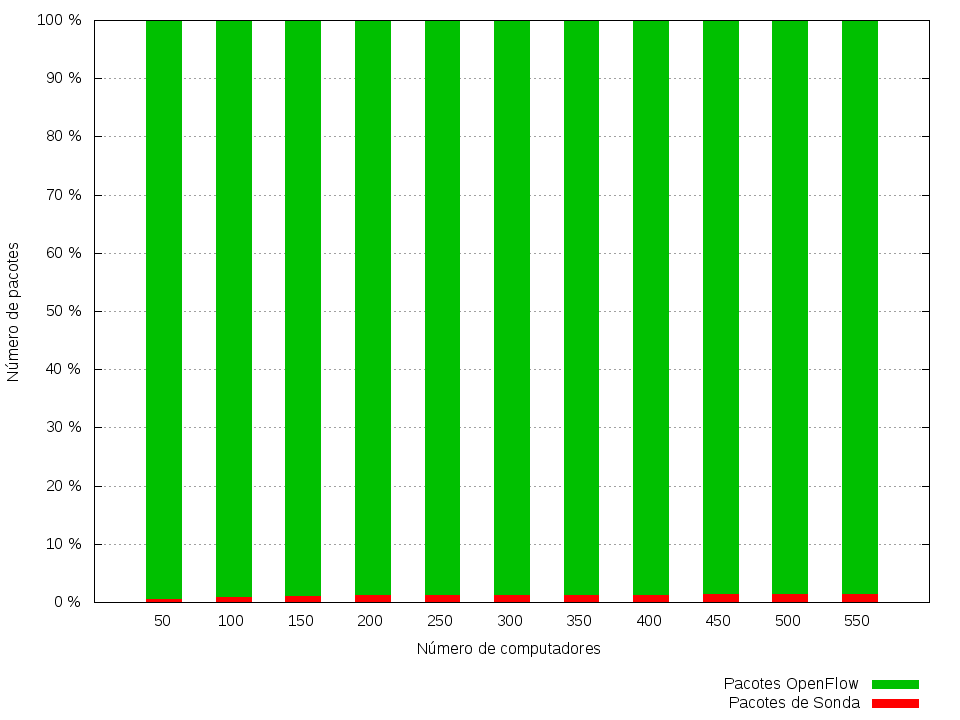
\includegraphics[width=\linewidth]{img/npings-x-packets-in-stacked}
    \caption{Valores percentuais do número de pacotes de sondagem e de 
        entrada manipulados pelo controlador}
\end{figure}

\section{Avaliação da rede}

Nesta seção são avaliados latência, largura de banda e \emph{jitter} da 
rede Ipê simulada.
Para cada cenário avaliado foram feitas comparações com e sem a presença 
do controlador com a solução em grafos. 
É avaliado o impacto da solução em grafos na rede.

\subsection{Avaliação de latência}

Em função do ambiente virtualizado, o experimento de latência foi dividido em 
duas partes.
A primeira avaliou a latência das redes locais.
Ou seja, a latência entre computadores de uma mesma subrede dentro de uma 
máquina virtual.
A segunda parte, avaliou a latência da rede global.
Ou seja, entre servidor físicos diferentes, fazendo com que os pacotes 
passem por toda a infraestrutura física do ambiente de simulação.
Para cada caso, foram medidos a latência com e sem o controlador em grafos.

Com a rede Ipê simulada completa foram executados, simultaneamente, 
6 pares de computadores enviando pacotes de ICMP PING. 
As medições da latência foram coletadas a cada segundo da execução do 
experimento. 
A latência em cada instante é a média de todos os 6 pares de computadores
a cada iteração de coleta.

\subsubsection{Latência da rede local}

A figura \ref{fig:local-latency} mostra a latência medida ao longo do 
experimento para as redes locais.
É possível notar que a latência da solução com controlador, no início do 
experimento, está em torno de 4 milisegundos.
Esse valor ocorre em função do encaminhamento, pelo comutador, do primeiro 
pacote para o controlador. 
Os valores subsequentes são próximos ao valor da latência medido na solução 
sem controlador.

\begin{figure}[!htb]
    \centering
    \label{fig:local-latency}
    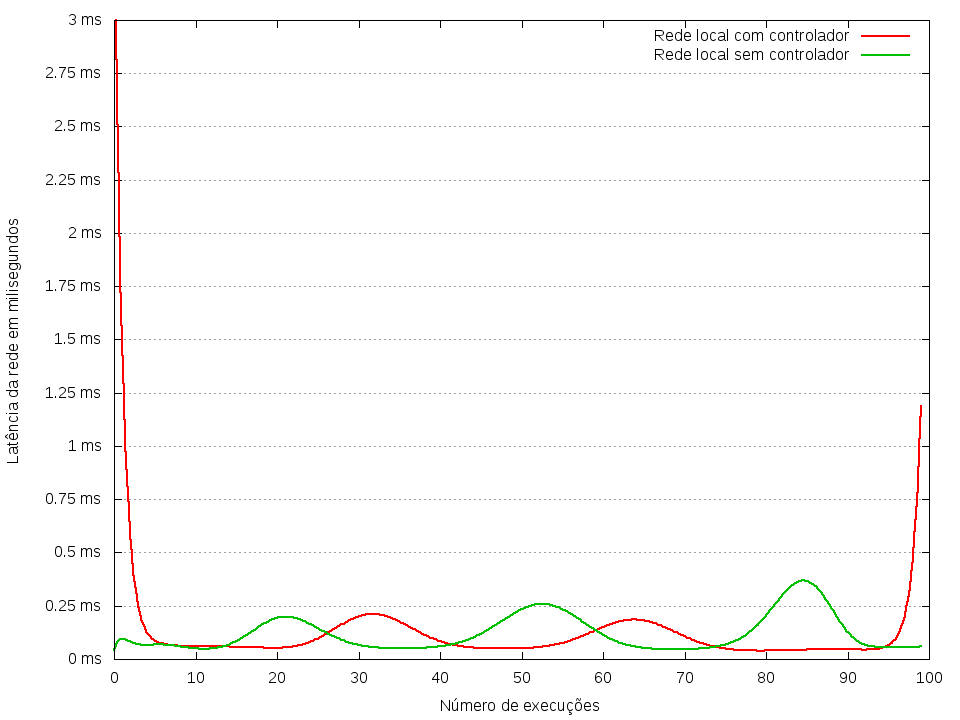
\includegraphics[width=\linewidth]{img/local-latency}
    \caption{Latência média das redes locais com e sem o controlador com a 
    solução em grafos}
\end{figure}

Uma avaliação dos dados coletados da largura de banda no ambiente das 
redes locais foi realizada.
Os valores de latência mínima, máxima e média com intervalo de confiança 
são apresentados na figura \ref{fig:local-latency-stats}.
No geral, as latências da rede com a solução do controlador em grafos e 
sem controlador se mantiveram parecidas. 
Em média, a latência no experimento das redes locais foi de 
$0,13$ milisegundos.
É possível notar através do intervalo de confiança que a latência na rede 
com o controlador se manteve mais constante ao longo do experimento.
Ou seja, mais confiável, com baixa variancia.

\begin{figure}[!htb]
    \centering
    \label{fig:local-latency-stats}
    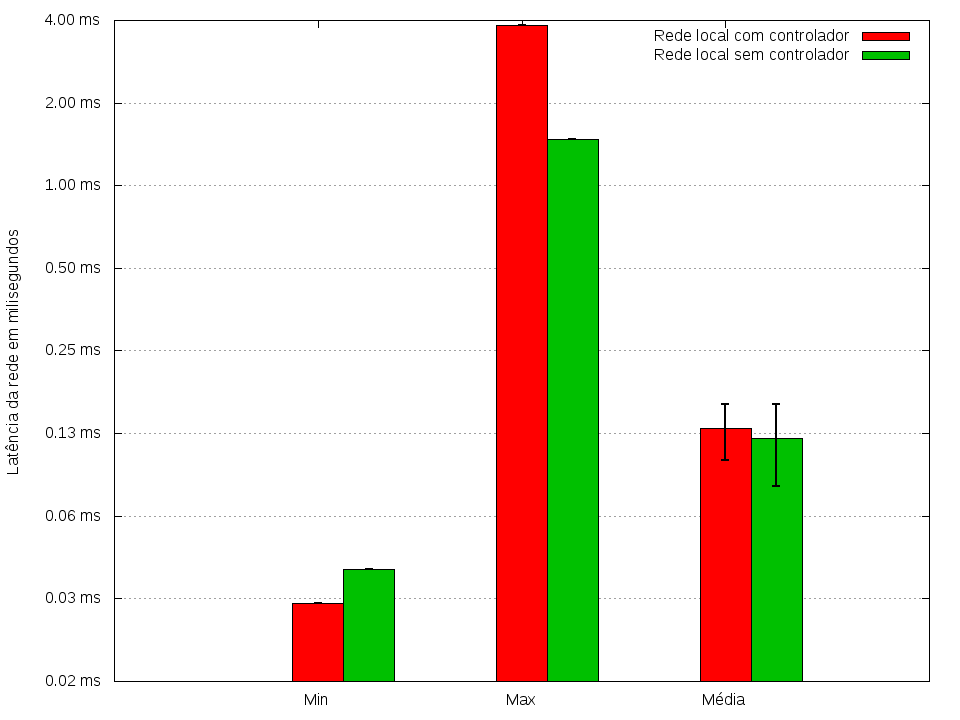
\includegraphics[width=\linewidth]{img/local-latency-stats}
    \caption{Latência mínima, máxima e média das redes locais}
\end{figure}


\subsubsection{Latência da rede global Ipê}

O mesmo perfil de experimento foi executado para o cenário da rede global.
6 pares de computadores executaram PINGs coletando os valores da latência
a cada segundo.
Para esse experimento, foram separados os pares em computadores diferentes 
para garantir que cada pacote trafegasse por toda infraestrutura física da 
rede simulada. 

A figura \ref{fig:ipe-latency} apresenta os resultados dessa avaliação.
Como pode ser visto, a latência inicial coletada na rede com a solução do 
controlador com o módulo grafo chegou a 400 milisegundos.
Esse valor ocorre em função do primeiro pacotes que é encaminhado para o 
controlador.
No geral, a latência da rede sem controlador sofreu uma variação mais alta.
Em contraponto a curva da latência com o controlador demonstra-se mais 
constante.

\begin{figure}[!htb]
    \centering
    \label{fig:ipe-latency}
    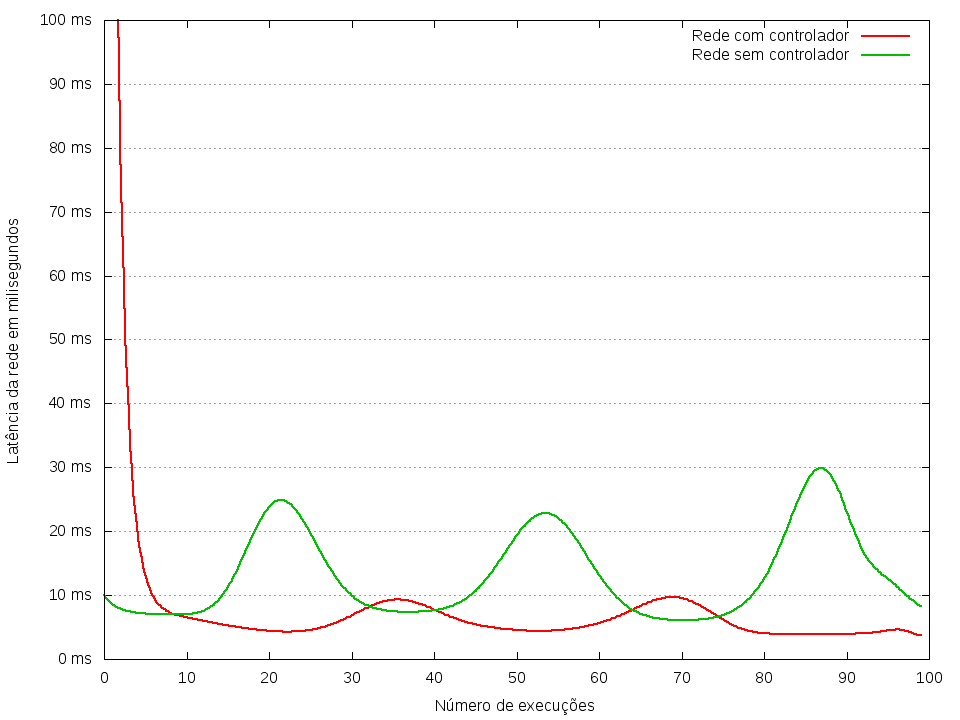
\includegraphics[width=\linewidth]{img/ipe-latency}
    \caption{Latência da rede Ipê com e sem o controlador com a solução em 
    grafos}
\end{figure}

Em média, a latência da rede Ipê simulada foi $13$ milisegundos.
Na rede global, o experimento sem controlador teve oscilações bem altas que
chegaram a valores de $100$ milisegundos de latência.
É possível notar novamente a estabilidade da rede com controlador observando
o desvio padrão mais baixo. 
A figura \ref{fig:ipe-latency-stats} apresenta os resultados da avaliação dos
valores mínimos, máximos e médios com desvio padrão da rede Ipê simulada.

Através dos experimento de latência realizados tanto nas redes locais quanto 
na rede Ipê global, pode-se notar que o controlador com a solução do módulo 
em grafos não gerou grande impacto na rede.
Com exceção dos primeiros pacotes, com uma latência alta, a rede com o 
controlador se mostrou mais estável do que sem. 

\begin{figure}[!htb]
    \centering
    \label{fig:ipe-latency-stats}
    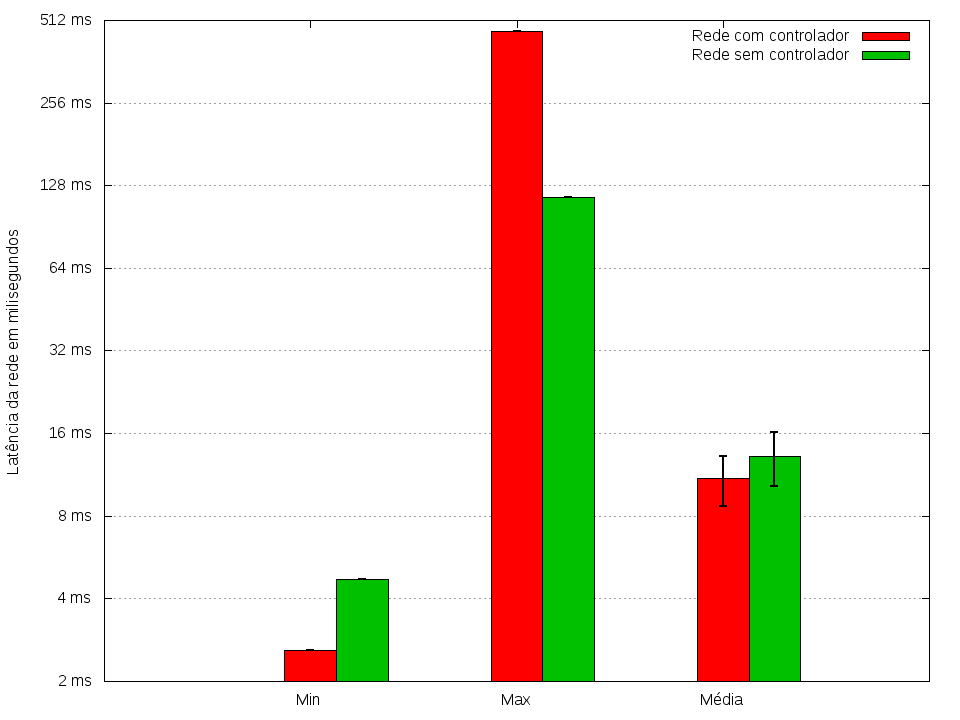
\includegraphics[width=\linewidth]{img/ipe-latency-stats}
    \caption{Avaliação da latência da rede Ipê considerando os valores mínimos,
    máximos e médios analisados}
\end{figure}

\subsection{Avaliação de largura de banda}

A avaliação da largura de banda foi feita utilizando 4 pares de computadores
em subredes e servidores da rede física diferentes.
Para cada par de computadores, foi utilizada a ferramenta de linha comando
\emph{iperf}.
O experimento consistiu em medir, com intervalos de 5 segundos, durante 
5 minutos, a largura de banda através de conexões TCP.
A largura de banda medida é representada pela média das quatro medições a
cada iteração de coleta durante o experimento.

A largura de banda da rede sem controlador medida durante o experimento foi, 
em média, $18$ \emph{Megabytes}.
Na figura \ref{fig:bandwidth-no-ctrl} são apresentados os resultados do 
experimento. 
Conforme pode ser visto nesta figura, os pontos representam os valores 
médios amostrados em todos os pares de computadores que estavam coletando 
a largura de banda.

\break

Uma interpolação suavizada e uma passando por todos os pontos médios mostram
a largura de banda média computada nesse experimento.

\begin{figure}[!htb]
    \centering
    \label{fig:bandwidth-no-ctrl}
    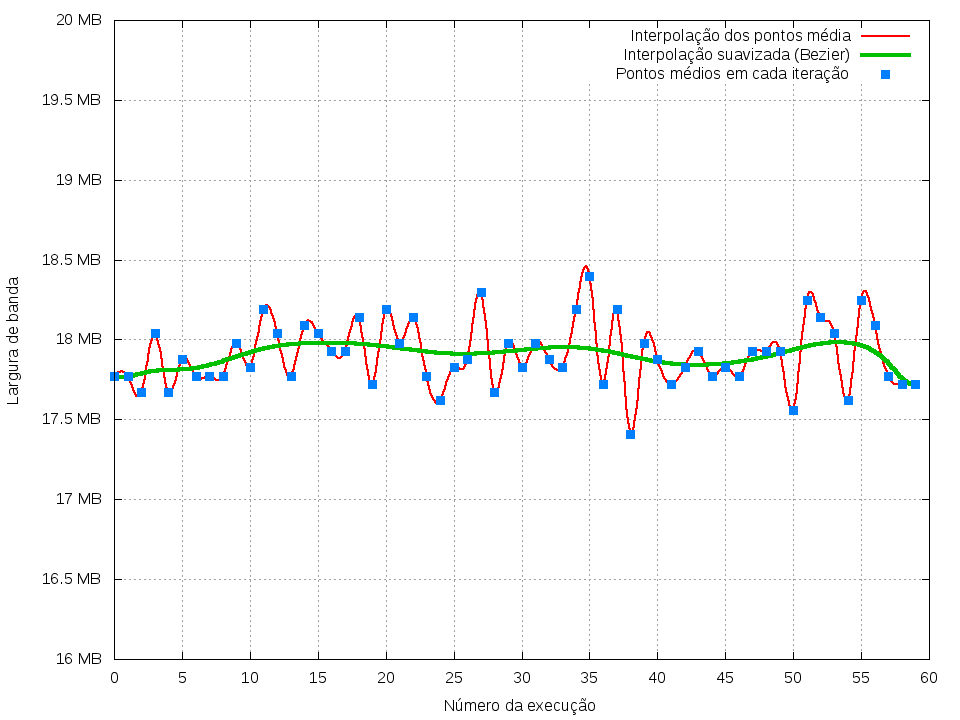
\includegraphics[width=\linewidth]{img/bandwidth-no-ctrl}
    \caption{Largura de banda média em \emph{Megabytes} da rede sem 
    controlador ao longo de 60 coletas}
\end{figure}

O mesmo experimento foi executado para a rede com o controlador utilizando 
a solução do módulo em grafos.
Para esse cenário, notou-se uma redução na largura de banda em função da 
utilização do \emph{OpenFlow} e o módulo em grafos.

A figura \ref{fig:bandwidth-ctrl} apresenta os resultados da largura de banda
média para o experimento com a solução em grafos.
A cada 5 segundos, uma nova conexão foi estabelecida entre cada par de 
computadores.

O primeiro pacote de cada conexão gerou um pacote de entrada \emph{PacketIn}.
Ao ser tratado pelo controlador, esses pacotes reduzem a fluidez da rede, pois
ocupam a CPU do controlador.
Pacotes na rede sem controlador não precisam ser processados por um computador
externo, logo não consomem da mesma forma a largura de banda.

\break

\begin{figure}[!htb]
    \centering
    \label{fig:bandwidth-ctrl}
    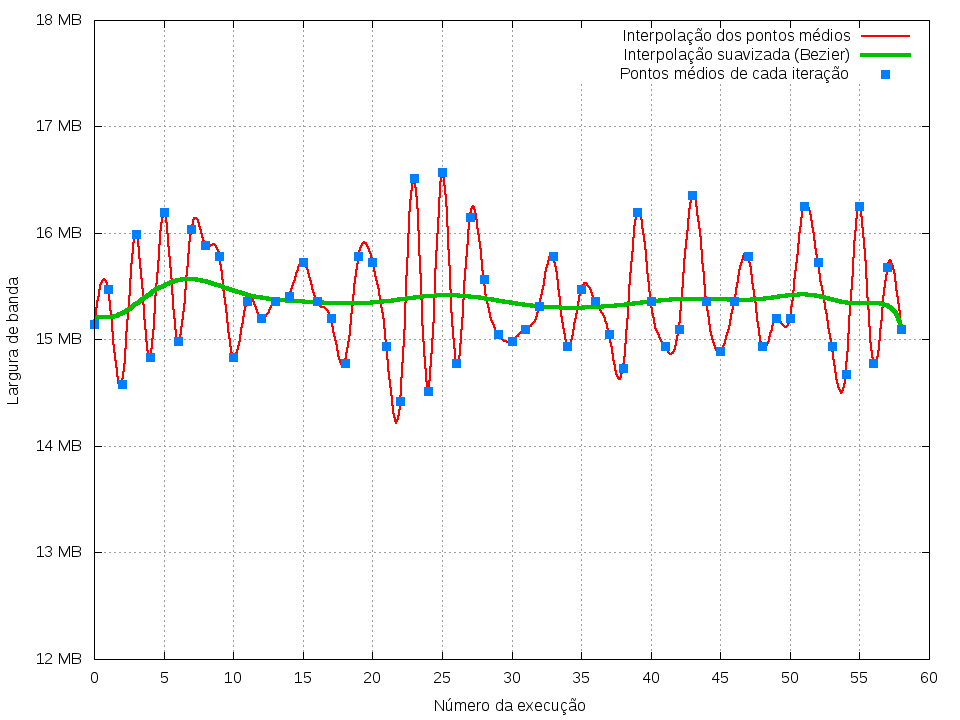
\includegraphics[width=\linewidth]{img/bandwidth-ctrl}
    \caption{Largura de banda média em \emph{Megabytes} da rede com o 
        controlador com a solução em grafos ao longo de 60 coletas}
\end{figure}

Como o tempo para processar os pacotes de entrada é sempre o mesmo, pode-se 
inferir que a redução da largura de banda se manteria a mesma em qualquer 
cenário.
Ou seja, em uma rede \emph{Gigabit} a diferença entre a largura de banda 
média com e sem controlador seria a mesma.

A figura \ref{fig:bandwidth-diff} apresenta a diferença entre as larguras de
banda média nos experimentos sem controlador e com o  módulo em grafos 
utilizando \emph{OpenFlow}.
A curva em vermelho representa a largura de banda média da rede sem 
controlador.
A curva em verde, a largura de banda da rede com controlador utilizando a 
solução em grafos.
As curvas representam a interpolação suavizada dos pontos médios computados
durante as 60 coletas realizadas durante o experimento.

Uma redução média de $2,5$ \emph{Megabytes} foi registrada durante o 
experimento da a rede sem controlador para a rede com controlador.

\begin{figure}[!htb]
    \centering
    \label{fig:bandwidth-diff}
    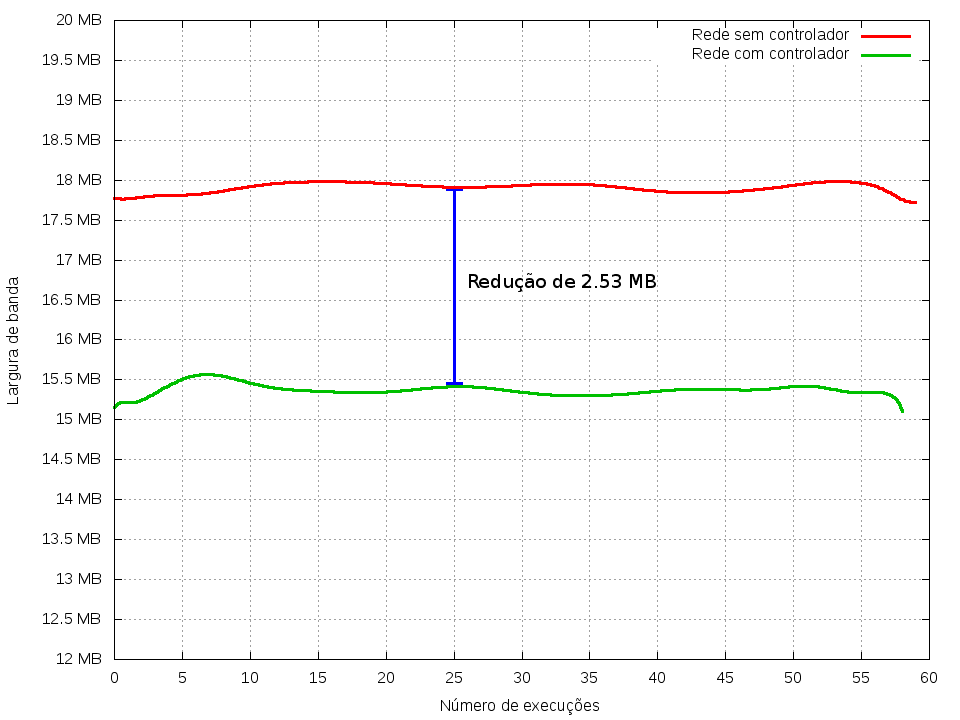
\includegraphics[width=\linewidth]{img/bandwidth-diff}
    \caption{Diferença da largura de banda dos experimento com e sem
    controlador}
\end{figure}



\subsection{Avaliação de \emph{jitter}}


\subsection{Avaliação de percentual de erros}




